\documentclass{itkmitlproject}

\usepackage{afterpage}
\usepackage{graphicx,amsmath,latexsym,amssymb,amsthm}
\usepackage{indentfirst}
\usepackage{hyperref}
\usepackage{hyphenat}
\usepackage[numbers,square]{natbib}
\usepackage{booktabs}
\usepackage{array}
\usepackage{tabularx}
\usepackage{longtable}

% \useEnglish
\useThai

\graphicspath{ {images/} }

%1. Your thesis title (THAI)
\newcommand{\ThesisTitle}{ระบบผู้ช่วยอัจฉริยะเพื่อการเรียนรู้และการติดตามนักศึกษาในระดับมหาวิทยาลัย}
%2. Your thesis title (ENG)
\newcommand{\ThesisTitleENG}{UniAssist AI: Intelligent Student Support and Advisor Monitoring System}
%3. Author name
\newcommand{\Author}{นางสาวนันท์ณภัส มะโนมั่น}
%4. Author name ENG
\newcommand{\AuthorENG}{Nannapas Manoman}
%5. Author student ID
\newcommand{\SId}{66070104}
%6. Author 2 name
\newcommand{\AuthorTwo}{นางสาวภาดาวัน โชติหิรัญคงวุฒิ}
%7. Author 2 name ENG
\newcommand{\AuthorTwoENG}{Padawan Chodhirunkongwut}
%8. Author 2 student ID
\newcommand{\SIdTwo}{66070154}
%9. Advisor name
\newcommand{\Advisor}{ดร.ภัทรภร วัฒนาชีพ}
%10. Advisor name ENG
\newcommand{\AdvisorENG}{Dr.Pattaraporn Wattanacheep}
%11. ภาคเรียนที่
\newcommand{\Sem}{2}
%12. ปีการศึกษา พ.ศ.
\newcommand{\AcaY}{2568}
%13. ปีการศึกษา ค.ศ.
\newcommand{\AcaYAD}{2025}
%14. วันส่งรายงาน
\newcommand{\SubD}{}
%15. Copyright year (AD)
\newcommand{\CopyrightYAD}{2025}

\begin{document}
    \frontmatter
    \lhead{}\rhead{}\chead{}\lfoot{}\cfoot{\thepage}\rfoot{}
    \makecover
    \makeinnercover
    \makeengcover
    \makecopyrightcover
    \makethesiscert
    \makeprojectcert

    % Setting margin for page numbering on frontmatter
    \newgeometry{top=1in, bottom=1in, left=1.5in, right=1in, includefoot}
    \setcounter{page}{1}
    \pagenumbering{Roman}

    \makeabstract{
        ปัจจุบันระบบการศึกษาในระดับมหาวิทยาลัยมีความซับซ้อน ทั้งโครงสร้างหลักสูตรและระเบียบข้อบังคับที่กระจายอยู่หลายแหล่ง ส่งผลให้นักศึกษาเข้าถึงข้อมูลได้ยากและเกิดความผิดพลาดในการวางแผนการเรียน โครงงานนี้จึงมุ่งพัฒนา \textbf{UniAssist AI} ซึ่งเป็นเว็บแอปพลิเคชันผู้ช่วยด้านวิชาการสำหรับนักศึกษาและอาจารย์ที่ปรึกษา คณะเทคโนโลยีสารสนเทศ สถาบันเทคโนโลยีพระจอมเกล้าเจ้าคุณทหารลาดกระบัง โดยให้บริการตอบคำถามข้อมูลหลักสูตรได้อย่างถูกต้องและรวดเร็ว

        การพัฒนาเริ่มจากการรวบรวมข้อมูลจากเอกสารหลักสูตร (มคอ.2) และตารางสอนของสำนักทะเบียน จากนั้นใช้โมเดลภาษาขนาดใหญ่ (LLM) สกัดข้อมูลที่มีโครงสร้างซับซ้อนให้อยู่ในรูปแบบข้อมูลเชิงสัมพันธ์ (Relational Database) และประเมินคุณภาพการสกัดเทียบกับเอกสาร มคอ.2 จริงบนโมเดล ๔ ตัว พบว่าโมเดล Qwen มีความสมดุลระหว่างความครบถ้วน (Coverage) และความถูกต้อง (Accuracy) สูงที่สุด จึงถูกเลือกเป็นโมเดลหลักของระบบ แกนหลักของระบบใช้เทคนิค \textbf{Text-to-SQL} คือให้ LLM แปลงคำถามภาษาไทยเป็นคำสั่ง SQL แล้วประมวลผลบนฐานข้อมูลแบบอ่านอย่างเดียว (read-only) พร้อมกลไกตรวจสอบความปลอดภัยของคำสั่งก่อนรัน และเรียบเรียงผลลัพธ์กลับเป็นภาษาที่เข้าใจง่าย นอกจากนี้ยังพัฒนาระบบคำนวณเกรดและประเมินความเสี่ยงทางการเรียนแบบอัตโนมัติ ระบบข้อมูลทุนการศึกษา และแดชบอร์ดสำหรับอาจารย์ที่ปรึกษา โดยมีการยืนยันตัวตนผ่าน Google OAuth และแบ่งสิทธิ์การใช้งานตามบทบาท

        ผลลัพธ์จากโครงงานนี้คือเว็บแอปพลิเคชันที่ช่วยให้นักศึกษาเข้าถึงข้อมูลและวางแผนการเรียนได้อย่างมีประสิทธิภาพ ลดความเสี่ยงในการพ้นสภาพนักศึกษา และช่วยให้อาจารย์ที่ปรึกษาติดตามสถานะของนักศึกษาในความดูแลได้อย่างทั่วถึง ซึ่งสอดคล้องกับเป้าหมายการพัฒนาที่ยั่งยืน (SDG 4) ในการส่งเสริมโอกาสการเรียนรู้และคุณภาพการศึกษา

        \vskip0.5cm
        \noindent\textbf{คำสำคัญ:} โมเดลภาษาขนาดใหญ่, Text-to-SQL, ผู้ช่วยด้านวิชาการ, การสกัดข้อมูลหลักสูตร, การประเมินความเสี่ยงทางการเรียน
    }

    \makeabstracteng{
        Higher-education systems are complex: curriculum structures and academic regulations are scattered across many sources, making it hard for students to access information and leading to mistakes in study planning. This project develops \textbf{UniAssist AI}, a web application that acts as an academic assistant for students and academic advisors at the School of Information Technology, King Mongkut's Institute of Technology Ladkrabang, providing accurate and fast answers to curriculum-related questions.

        Development began by collecting data from curriculum documents (TQF2 / \emph{มคอ.2}) and the registrar's teaching timetable. A Large Language Model (LLM) was then used to extract this highly structured information into a relational database. The extraction quality was evaluated against the official curriculum documents across four models; the Qwen model achieved the best balance between coverage and accuracy and was therefore selected as the system's primary model. The core of the system uses a \textbf{Text-to-SQL} technique: the LLM translates Thai natural-language questions into SQL statements that are executed on a read-only database, with a safety-checking mechanism applied before execution, and the results are then paraphrased back into easy-to-understand language. In addition, the system provides automatic GPA calculation with academic-risk assessment, a scholarship information module, and a dashboard for academic advisors, with authentication via Google OAuth and role-based access control.

        The result is a web application that helps students access information and plan their studies effectively, reduces the risk of academic dismissal, and enables academic advisors to monitor the students under their supervision comprehensively, in line with Sustainable Development Goal 4 (Quality Education).

        \vskip0.5cm
        \noindent\textbf{Keywords:} Large Language Model, Text-to-SQL, Academic Assistant, Curriculum Data Extraction, Academic Risk Assessment
    }

    \makeack

    \newpage
    \addcontentsline{toc}{chapter}{\contentsname}
    \tableofcontents

    \newpage
    \addcontentsline{toc}{chapter}{\listtablename}
    \listoftables

    \newpage
    \addcontentsline{toc}{chapter}{\listfigurename}
    \listoffigures

    % Reset frontmatter page numbering margin, back to original margin from class file
    \restoregeometry

    \mainmatter
    \lhead{}\rhead{\thepage}\chead{}\lfoot{}\cfoot{}\rfoot{}

    \chapter{บทนำ}
\label{chapter:introduction}

\section{ที่มาและความสำคัญ}

ในระดับมหาวิทยาลัย ระบบการเรียนการสอนมีความซับซ้อนมากกว่าระดับมัธยมศึกษาอย่างมีนัยสำคัญ ทั้งในด้านโครงสร้างหลักสูตร การลงทะเบียนเรียน ระเบียบข้อบังคับทางวิชาการ การคำนวณผลการเรียน และขั้นตอนทางวิชาการต่าง ๆ ความซับซ้อนดังกล่าวส่งผลให้นักศึกษา โดยเฉพาะนักศึกษาใหม่ ประสบความยากลำบากในการทำความเข้าใจระบบการเรียนและการปรับตัวในช่วงเริ่มต้นของการศึกษาในระดับมหาวิทยาลัย

นอกจากนี้ ข้อมูลสำคัญทางการศึกษาของมหาวิทยาลัยมักกระจัดกระจายอยู่ในหลายแหล่ง เช่น เว็บไซต์สำนักทะเบียน ประกาศข่าวสาร เอกสารในรูปแบบไฟล์ PDF และเอกสารจากคณะหรือภาควิชา ทำให้การเข้าถึงข้อมูลเป็นไปได้ยาก ข้อมูลบางส่วนอาจไม่เป็นปัจจุบันหรือสูญหาย ส่งผลให้นักศึกษาเกิดความสับสนและอาจตัดสินใจผิดพลาด เช่น การลงทะเบียนเรียนไม่เป็นไปตามลำดับของหลักสูตร หรือการอ้างอิงระเบียบการศึกษาที่ไม่ตรงกับปีการศึกษาที่ตนสังกัด

ในด้านข้อมูลวิชาการ รายละเอียดเกี่ยวกับผังหลักสูตร รายวิชาเลือกเสรี และรายวิชาบังคับก่อนเรียน (Prerequisite) มักถูกเขียนในลักษณะเป็นทางการและมีความซับซ้อน ทำให้นักศึกษาบางส่วนตีความข้อมูลผิดพลาด และเลือกลงทะเบียนในรายวิชาที่ไม่สามารถลงเรียนได้จริง ส่งผลกระทบต่อแผนการเรียนและระยะเวลาการศึกษา

ขณะเดียวกัน ปัญหาเกี่ยวกับการคำนวณผลการเรียนและการประเมินความเสี่ยงต่อการพ้นสภาพการเป็นนักศึกษายังคงเป็นประเด็นสำคัญ นักศึกษาจำนวนมากไม่เข้าใจเกณฑ์คะแนนเฉลี่ยสะสมขั้นต่ำ (GPA) หรือเงื่อนไขการพ้นสภาพ ทำให้ไม่สามารถประเมินสถานะทางการเรียนของตนเองได้อย่างถูกต้อง ส่งผลให้ขาดการวางแผนแก้ไขปัญหาล่วงหน้า

สำหรับอาจารย์ที่ปรึกษา การติดตามและดูแลนักศึกษาก็เป็นไปอย่างจำกัด เนื่องจากข้อมูลที่เกี่ยวข้องกับผลการเรียนและความเสี่ยงของนักศึกษากระจายอยู่ในหลายระบบ และขาดเครื่องมือที่สามารถสรุปภาพรวมของนักศึกษาได้อย่างมีประสิทธิภาพ ส่งผลให้การให้คำปรึกษามักเกิดขึ้นหลังจากนักศึกษาเผชิญกับปัญหาแล้ว

จากปัญหาดังกล่าว จึงมีความจำเป็นในการพัฒนา \textbf{UniAssist AI} ที่สามารถรวบรวมข้อมูลทางการศึกษาของมหาวิทยาลัยไว้ในศูนย์กลางเดียว อธิบายข้อมูลที่มีความซับซ้อนให้อยู่ในรูปแบบที่เข้าใจง่าย ให้คำแนะนำด้านวิชาการอย่างถูกต้อง ประเมินความเสี่ยงทางการเรียนของนักศึกษาแบบเรียลไทม์ และสนับสนุนการทำงานของอาจารย์ที่ปรึกษาในการติดตามและดูแลนักศึกษาได้อย่างมีประสิทธิภาพมากยิ่งขึ้น

ในการพัฒนาระบบตอบคำถามนั้น เนื่องจากข้อมูลหลักสูตรของคณะมีลักษณะเป็นข้อมูลที่มีโครงสร้างชัดเจน (เช่น รายวิชา หน่วยกิต ปี/ภาคการศึกษา และเงื่อนไขบังคับก่อน) โครงงานนี้จึงเลือกจัดเก็บข้อมูลในรูปแบบฐานข้อมูลเชิงสัมพันธ์ (Relational Database) และประยุกต์ใช้เทคนิค \textbf{Text-to-SQL} ซึ่งให้โมเดลภาษาขนาดใหญ่ (Large Language Model: LLM) แปลงคำถามภาษาไทยของผู้ใช้ให้เป็นคำสั่ง SQL เพื่อค้นคืนข้อมูลจากฐานข้อมูลโดยตรง แนวทางนี้ทำให้คำตอบอ้างอิงจากข้อมูลจริงในฐานข้อมูลของคณะ ลดปัญหาการสร้างข้อมูลเท็จ (Hallucination) และสามารถตรวจสอบย้อนกลับได้ว่าคำตอบมาจากคำสั่งค้นข้อมูลใด

\section{วัตถุประสงค์}

\begin{enumerate}
    \item เพื่อพัฒนาระบบผู้ช่วยด้านการศึกษา (AI Education Assistant) ที่รวบรวมข้อมูลทางการศึกษาของคณะเทคโนโลยีสารสนเทศจากหลายแหล่งให้อยู่ในฐานข้อมูลเดียว เพื่อให้นักศึกษาเข้าถึงข้อมูลที่ถูกต้องและเป็นปัจจุบันได้อย่างสะดวก
    \item เพื่อพัฒนา AI Chatbot ด้านวิชาการที่ตอบคำถามของนักศึกษาได้ตลอด 24 ชั่วโมง โดยประยุกต์ใช้เทคนิค Text-to-SQL ร่วมกับความสามารถในการให้เหตุผลของโมเดลภาษาขนาดใหญ่ (LLM Reasoning) เพื่อเพิ่มความแม่นยำและความเข้าใจง่ายของคำตอบ พร้อมทั้งลดปัญหาการให้ข้อมูลเท็จ
    \item เพื่อออกแบบระบบคำนวณผลการเรียนและประเมินความเสี่ยงทางการศึกษาโดยอัตโนมัติ เช่น ความเสี่ยงต่อการพ้นสภาพการเป็นนักศึกษา พร้อมทั้งให้คำแนะนำเชิงปฏิบัติแก่นักศึกษาได้อย่างทันท่วงที
    \item เพื่อพัฒนาระบบข้อมูลทุนการศึกษาและข้อมูลด้านการเงิน พร้อมช่วยวิเคราะห์คุณสมบัติเบื้องต้นของนักศึกษาเทียบกับเงื่อนไขการสมัครทุน
    \item เพื่อสนับสนุนการทำงานของอาจารย์ที่ปรึกษา โดยจัดให้มีแดชบอร์ดติดตามผลการเรียนและการประเมินความเสี่ยงของนักศึกษาในความดูแล เพื่อเพิ่มประสิทธิภาพในการให้คำปรึกษาทางวิชาการ
    \item เพื่อส่งเสริมเป้าหมายการพัฒนาที่ยั่งยืน SDG 4: คุณภาพการศึกษา โดยเพิ่มความเท่าเทียมในการเข้าถึงข้อมูลทางการศึกษา ส่งเสริมการวางแผนการเรียนอย่างเป็นระบบ และช่วยลดปัญหาการเรียนล่าช้าในระดับอุดมศึกษา
\end{enumerate}

\section{วิธีการดำเนินงาน}

\begin{enumerate}
    \item \textbf{การตั้งปัญหาและวิเคราะห์ความต้องการของระบบ} วิเคราะห์ปัญหาและความต้องการของนักศึกษาและอาจารย์ที่ปรึกษา เช่น การเข้าถึงข้อมูลการศึกษา การวางแผนการเรียน ทุนการศึกษา และการติดตามความเสี่ยง เพื่อกำหนดขอบเขตและฟังก์ชันของระบบ
    \item \textbf{การรวบรวมและจัดเตรียมข้อมูล} รวบรวมข้อมูลทางการศึกษาจากเอกสารหลักสูตร (มคอ.2) ผังหลักสูตร ระเบียบการศึกษา และตารางสอนจากสำนักทะเบียน จากนั้นใช้โมเดลภาษาขนาดใหญ่สกัดข้อมูลที่มีโครงสร้างซับซ้อนให้อยู่ในรูปแบบข้อมูลที่มีโครงสร้าง (Structured Data) และจัดเก็บลงในฐานข้อมูลเชิงสัมพันธ์
    \item \textbf{การประเมินคุณภาพการสกัดข้อมูล} เปรียบเทียบผลการสกัดข้อมูลจากโมเดลภาษาหลายตัว (Qwen, Gemini, DeepSeek และ Typhoon) กับเอกสารหลักสูตรฉบับจริง เพื่อคัดเลือกโมเดลที่เหมาะสมที่สุดสำหรับสร้างฐานข้อมูลและใช้งานในระบบ
    \item \textbf{การพัฒนาแกน Text-to-SQL Chatbot} พัฒนาแกนการทำงานที่ให้ LLM แปลงคำถามภาษาไทยเป็นคำสั่ง SQL รันบนฐานข้อมูลแบบอ่านอย่างเดียว ผ่านกลไกตรวจสอบความปลอดภัยของคำสั่ง แล้วเรียบเรียงผลลัพธ์กลับเป็นภาษาที่เข้าใจง่าย
    \item \textbf{การพัฒนาระบบคำนวณเกรดและประเมินความเสี่ยง} พัฒนาระบบคำนวณผลการเรียนและประเมินความเสี่ยงของนักศึกษาโดยอัตโนมัติ โดยอ้างอิงกฎเกณฑ์ของสถาบันที่จัดเก็บในฐานข้อมูล และใช้ LLM สรุปสถานะและให้คำแนะนำเชิงปฏิบัติ
    \item \textbf{การพัฒนาระบบทุนการศึกษาและแดชบอร์ดอาจารย์} พัฒนาระบบให้ข้อมูลทุนการศึกษาและวิเคราะห์คุณสมบัติเบื้องต้น และพัฒนาแดชบอร์ดสำหรับอาจารย์ที่ปรึกษาเพื่อแสดงภาพรวมผลการเรียนและความเสี่ยงของนักศึกษา
    \item \textbf{การพัฒนาส่วนติดต่อผู้ใช้และระบบยืนยันตัวตน} พัฒนาเว็บแอปพลิเคชันและระบบยืนยันตัวตนผ่าน Google OAuth พร้อมแบ่งสิทธิ์การใช้งานตามบทบาท (นักศึกษา / อาจารย์ที่ปรึกษา / ผู้พัฒนา)
    \item \textbf{การพัฒนาและทดสอบระบบ} พัฒนาระบบในรูปแบบเว็บแอปพลิเคชันและดำเนินการทดสอบด้านความถูกต้องของข้อมูล การคำนวณเกรด และการตอบคำถามของ AI Chatbot เพื่อปรับปรุงระบบให้มีความน่าเชื่อถือ
\end{enumerate}

\section{ขอบเขตของโครงงาน}

\begin{enumerate}
    \item พัฒนาและรวบรวมข้อมูลด้านการศึกษาที่เกี่ยวข้องกับคณะเทคโนโลยีสารสนเทศทุกหลักสูตรในระดับปริญญาตรี (IT, DSBA, BIT และ AIT) ของสถาบันเทคโนโลยีพระจอมเกล้าเจ้าคุณทหารลาดกระบัง โดยดึงข้อมูลจากแหล่งข้อมูลที่เกี่ยวข้อง เช่น เอกสารหลักสูตร มคอ.2 ผังหลักสูตร ระเบียบการศึกษา และตารางสอนของสำนักทะเบียน
    \item พัฒนาระบบ AI Chatbot ด้านการศึกษาสำหรับนักศึกษาคณะเทคโนโลยีสารสนเทศ เพื่อตอบคำถามด้านการเรียน การลงทะเบียน ผังหลักสูตร และระเบียบการศึกษา โดยประยุกต์ใช้เทคนิค Text-to-SQL ร่วมกับความสามารถในการให้เหตุผลของโมเดลภาษาขนาดใหญ่
    \item ออกแบบและพัฒนาระบบคำนวณผลการเรียนและประเมินความเสี่ยงทางการศึกษาของนักศึกษา เช่น ความเสี่ยงต่อการพ้นสภาพการเป็นนักศึกษา โดยอ้างอิงตามเกณฑ์และข้อบังคับของสถาบัน
    \item พัฒนาระบบข้อมูลทุนการศึกษา เพื่อให้ข้อมูลเกี่ยวกับเงื่อนไขและคุณสมบัติการสมัครทุน พร้อมช่วยวิเคราะห์คุณสมบัติเบื้องต้นของนักศึกษา
    \item ออกแบบและพัฒนาแดชบอร์ดสำหรับอาจารย์ที่ปรึกษา เพื่อติดตามข้อมูลผลการเรียน วิเคราะห์ความเสี่ยง และสนับสนุนการให้คำแนะนำทางการศึกษาแก่นักศึกษาในความดูแล
    \item ออกแบบและพัฒนาส่วนติดต่อผู้ใช้ (UX/UI) ของเว็บแอปพลิเคชัน พร้อมระบบยืนยันตัวตนและการควบคุมสิทธิ์การเข้าถึงตามบทบาทผู้ใช้
    \item พัฒนาและทดสอบระบบในรูปแบบเว็บแอปพลิเคชัน โดยทดสอบความถูกต้องของข้อมูล การคำนวณผลการเรียน และการตอบคำถามของ AI Chatbot เพื่อประเมินประสิทธิภาพและปรับปรุงระบบให้เหมาะสมกับการใช้งานจริง
\end{enumerate}

\section{ประโยชน์ที่คาดว่าจะได้รับ}

\begin{enumerate}
    \item นักศึกษาสามารถติดตามข่าวสารและข้อมูลด้านการศึกษาได้อย่างรวดเร็ว และสอบถามข้อสงสัยต่าง ๆ ได้ทันทีผ่านระบบเดียว
    \item อาจารย์ที่ปรึกษาสามารถติดตามและดูแลนักศึกษาได้อย่างมีประสิทธิภาพ และรับรู้สถานะการเรียนและความเสี่ยงของนักศึกษาได้
    \item นักศึกษาสามารถวางแผนการเรียนและเลือกลงทะเบียนรายวิชาได้อย่างราบรื่นและสะดวกมากยิ่งขึ้น
    \item AI Chatbot ที่พัฒนาขึ้นสามารถตอบคำถามด้านการศึกษาได้อย่างถูกต้อง ไม่สร้างข้อมูลเท็จ และอ้างอิงจากข้อมูลจริงของคณะโดยตรง
    \item ระบบช่วยส่งเสริมการเข้าถึงข้อมูลด้านการศึกษาอย่างง่ายดาย เท่าเทียม และทั่วถึง สอดคล้องกับเป้าหมายการพัฒนาที่ยั่งยืน SDG 4 ด้านคุณภาพการศึกษา
\end{enumerate}

\section{ศัพท์นิยามเฉพาะ}

\begin{enumerate}
    \item \textbf{Large Language Model (LLM)} โมเดลภาษาขนาดใหญ่ที่ผ่านการฝึกฝนด้วยข้อมูลจำนวนมหาศาล มีความสามารถในการเข้าใจ ตีความ และสร้างข้อความภาษามนุษย์ รวมถึงมีความสามารถในการให้เหตุผล (Reasoning)
    \item \textbf{Text-to-SQL} เทคนิคการแปลงคำถามภาษาธรรมชาติ (Natural Language) ให้เป็นคำสั่งภาษา SQL โดยอัตโนมัติ เพื่อค้นคืนข้อมูลจากฐานข้อมูลเชิงสัมพันธ์ตามความต้องการของผู้ใช้
    \item \textbf{Relational Database} ฐานข้อมูลเชิงสัมพันธ์ที่จัดเก็บข้อมูลในรูปแบบตารางที่มีความสัมพันธ์กัน และเข้าถึงด้วยภาษา SQL ในโครงงานนี้ใช้ระบบจัดการฐานข้อมูล SQLite
    \item \textbf{Retrieval-Augmented Generation (RAG)} เทคนิคที่เพิ่มประสิทธิภาพให้แก่โมเดลภาษาโดยการค้นคืนข้อมูลที่เกี่ยวข้องจากฐานความรู้ภายนอกมาประกอบการสร้างคำตอบ เพื่อลดการให้ข้อมูลเท็จและทำให้ข้อมูลเป็นปัจจุบัน
    \item \textbf{Prerequisite (รายวิชาบังคับก่อน)} รายวิชาพื้นฐานหรือเงื่อนไขที่นักศึกษาจำเป็นต้องลงทะเบียนเรียนและสอบผ่านตามเกณฑ์ที่กำหนด ก่อนที่จะมีสิทธิ์ลงทะเบียนในรายวิชาต่อเนื่องหรือรายวิชาในระดับที่สูงขึ้นตามผังหลักสูตร
    \item \textbf{Academic Dismissal (การพ้นสภาพการเป็นนักศึกษา)} สถานะทางการศึกษาที่สิ้นสุดลงเนื่องจากนักศึกษามีผลการเรียนเฉลี่ยสะสม (GPA) ต่ำกว่าเกณฑ์ขั้นต่ำที่สถาบันกำหนด หรือไม่ปฏิบัติตามเงื่อนไขการศึกษาระหว่างที่เป็นนักศึกษา
    \item \textbf{Hallucination} ปรากฏการณ์ที่โมเดลภาษาสร้างคำตอบที่ฟังดูสมเหตุสมผลแต่ไม่สอดคล้องกับข้อเท็จจริงหรือไม่มีแหล่งอ้างอิงจริง
    \item \textbf{OAuth} มาตรฐานการมอบสิทธิ์ (Authorization) ที่อนุญาตให้แอปพลิเคชันยืนยันตัวตนผู้ใช้ผ่านผู้ให้บริการภายนอก (เช่น Google) โดยไม่ต้องจัดเก็บรหัสผ่านของผู้ใช้เอง
    \item \textbf{มคอ.2} เอกสารรายละเอียดของหลักสูตร (Program Specification) ตามกรอบมาตรฐานคุณวุฒิระดับอุดมศึกษาแห่งชาติ (TQF) ซึ่งระบุโครงสร้างหลักสูตร รายวิชา หน่วยกิต และผลการเรียนรู้ที่คาดหวัง
    \item \textbf{SDG 4 (Sustainable Development Goal 4)} เป้าหมายการพัฒนาที่ยั่งยืนข้อที่ 4 ของสหประชาชาติ ว่าด้วยการสร้างหลักประกันว่าทุกคนมีการศึกษาที่มีคุณภาพอย่างครอบคลุมและเท่าเทียม
\end{enumerate}

    \chapter{การทบทวนวรรณกรรมที่เกี่ยวข้อง}
\label{chapter:literature-review}

ในการพัฒนา UniAssist AI ระบบผู้ช่วยอัจฉริยะเพื่อการเรียนรู้และการติดตามนักศึกษา คณะผู้จัดทำได้ศึกษาทฤษฎีและบทความวิจัยที่เกี่ยวข้อง เพื่อให้ระบบสามารถทำงานได้อย่างมีประสิทธิภาพ แม่นยำ และตอบโจทย์ผู้ใช้งาน โดยแบ่งหัวข้อการศึกษาออกเป็นสองส่วน ได้แก่ ทฤษฎีที่เกี่ยวข้อง และบทความวิจัยที่เกี่ยวข้อง

\section{ทฤษฎีที่เกี่ยวข้อง}

\subsection{โมเดลภาษาขนาดใหญ่ (Large Language Model: LLM)}

โมเดลภาษาขนาดใหญ่คือโมเดลปัญญาประดิษฐ์ประเภทการเรียนรู้เชิงลึก (Deep Learning) ที่ได้รับการฝึกฝนด้วยข้อมูลข้อความจำนวนมหาศาล โดยมีพื้นฐานมาจากสถาปัตยกรรมแบบ Transformer ซึ่งอาศัยกลไก Self-Attention ในการเรียนรู้ความสัมพันธ์ระหว่างคำในบริบท \cite{vaswani2017attention} ทำให้มีความสามารถในการเข้าใจบริบททางภาษา การสรุปความ และการสร้างข้อความที่ใกล้เคียงกับมนุษย์ ในโครงงานนี้มีการศึกษาเรื่องการออกแบบคำสั่ง (Prompt Engineering) และการให้เหตุผลของโมเดล (LLM Reasoning) เพื่อนำมาประยุกต์ใช้ในการวิเคราะห์เจตนาของคำถาม (Intent Recognition) การแปลงคำถามเป็นคำสั่ง SQL และการให้เหตุผลเกี่ยวกับกฎระเบียบการลงทะเบียนเรียนที่ซับซ้อน

\subsection{การแปลงภาษาธรรมชาติเป็นคำสั่ง SQL (Text-to-SQL)}

Text-to-SQL หรือ NL2SQL คือกระบวนการแปลงคำถามภาษาธรรมชาติให้เป็นคำสั่งภาษา SQL โดยอัตโนมัติ เพื่อให้ผู้ใช้ที่ไม่มีความรู้ด้านฐานข้อมูลสามารถสอบถามข้อมูลจากฐานข้อมูลเชิงสัมพันธ์ได้ กระบวนการนี้ต้องอาศัยความเข้าใจทั้งความหมายของคำถาม (Semantics) และโครงสร้างของฐานข้อมูล (Schema) ในอดีตงานด้านนี้ใช้แบบจำลองที่ฝึกเฉพาะทางบนชุดข้อมูลมาตรฐาน เช่น WikiSQL และ Spider \cite{yu2018spider} แต่ในปัจจุบันโมเดลภาษาขนาดใหญ่ที่มีความสามารถในการให้เหตุผลสามารถสร้างคำสั่ง SQL ได้อย่างมีประสิทธิภาพผ่านการให้บริบทของ schema และตัวอย่างในคำสั่ง (In-context Learning) โดยไม่จำเป็นต้องฝึกโมเดลใหม่ ข้อได้เปรียบของแนวทาง Text-to-SQL เมื่อเทียบกับการให้ LLM ตอบจากความจำโดยตรง คือคำตอบจะถูกดึงจากข้อมูลจริงในฐานข้อมูล ทำให้ตรวจสอบย้อนกลับได้และลดปัญหาการสร้างข้อมูลเท็จ เนื่องจากข้อมูลหลักสูตรมีลักษณะเป็นข้อมูลที่มีโครงสร้างชัดเจน แนวทางนี้จึงมีความเหมาะสมสำหรับการค้นคืนข้อมูลเชิงข้อเท็จจริง เช่น รายวิชา หน่วยกิต และเงื่อนไขบังคับก่อน

\subsection{การสร้างข้อความโดยอาศัยการค้นคืนข้อมูล (Retrieval-Augmented Generation: RAG)}

RAG \cite{lewis2020rag} คือกระบวนการที่ช่วยเพิ่มความแม่นยำให้กับโมเดลภาษา โดยการเชื่อมต่อโมเดลเข้ากับฐานความรู้ภายนอก (External Knowledge Base) เช่น คู่มือนักศึกษา หรือระเบียบการลงทะเบียน กระบวนการทำงานประกอบด้วย 3 ส่วนหลัก คือ (1) Retrieve ค้นหาเอกสารที่เกี่ยวข้องกับคำถามจากฐานข้อมูล (2) Augment นำข้อมูลที่ค้นพบมารวมกับคำถามตั้งต้น และ (3) Generate ส่งข้อมูลทั้งหมดให้ LLM ประมวลผลเพื่อสร้างคำตอบ เทคนิคนี้ช่วยลดปัญหาการตอบข้อมูลเท็จ (Hallucination) และทำให้ข้อมูลมีความเป็นปัจจุบัน ในโครงงานนี้แนวคิด RAG ถูกนำมาใช้เป็นกรอบความคิดเชิงหลักการของการ ``ตอบคำถามโดยยึดจากข้อมูลจริง'' โดยแนวทาง Text-to-SQL ที่นำมาใช้ถือเป็นรูปแบบหนึ่งของการค้นคืนข้อมูลที่เหมาะกับข้อมูลเชิงโครงสร้าง ขณะที่โหมดสนทนาทั่วไปของระบบใช้การยึดข้อมูล (Grounding) จากสรุปข้อเท็จจริงในฐานข้อมูลเพื่อลดการตอบนอกบริบท

\subsection{ฐานข้อมูลเชิงเวกเตอร์และการฝังคำ (Vector Database \& Text Embedding)}

ทฤษฎีการแปลงข้อมูลข้อความให้อยู่ในรูปแบบของตัวเลขหรือเวกเตอร์ (Vector Embeddings) เพื่อให้คอมพิวเตอร์สามารถเข้าใจความหมายเชิงบริบท (Semantic Meaning) ของข้อความได้ การใช้งานฐานข้อมูลเชิงเวกเตอร์ช่วยให้ระบบสามารถค้นหาข้อมูลที่มีความหมายใกล้เคียงกัน (Semantic Search) ได้อย่างมีประสิทธิภาพ แม้ว่าผู้ใช้งานจะใช้คำศัพท์ที่ไม่ตรงกับเอกสารต้นฉบับก็ตาม แนวคิดนี้เหมาะกับข้อมูลที่ไม่มีโครงสร้างชัดเจน (เช่น ประกาศหรือคู่มือแบบข้อความยาว) และเป็นแนวทางที่โครงงานพิจารณาไว้สำหรับการต่อยอดในการค้นคืนข้อมูลกฎระเบียบเชิงบรรยายในอนาคต

\subsection{ระบบแนะนำข้อมูล (Recommender System)}

การศึกษาระบบแนะนำเพื่อนำมาประยุกต์ใช้ในการแนะนำรายวิชา (Course Recommendation) โดยในโครงงานนี้มุ่งเน้นศึกษาระบบแนะนำที่อิงตามความรู้และข้อจำกัด (Knowledge-based / Constraint-based Recommender System) เนื่องจากเงื่อนไขการลงทะเบียนเรียนมีความซับซ้อนและมีกฎเกณฑ์ตายตัว (เช่น รายวิชาบังคับก่อน หรือ Prerequisite) ระบบจึงต้องวิเคราะห์ความต้องการของผู้เรียนร่วมกับโครงสร้างหลักสูตรเพื่อเสนอทางเลือกที่เหมาะสมที่สุด

\subsection{การทำเหมืองข้อมูลทางการศึกษา (Educational Data Mining: EDM)}

EDM คือศาสตร์ที่ประยุกต์ใช้เทคนิคการทำเหมืองข้อมูล (Data Mining) กับข้อมูลทางการศึกษา เพื่อค้นหารูปแบบความสัมพันธ์ที่ซ่อนอยู่ ในโครงงานนี้ได้ศึกษาเทคนิคการวิเคราะห์ข้อมูลผลการเรียน (Grade Analysis) และการประเมินความเสี่ยง (Risk Assessment) โดยใช้การกำหนดกฎเกณฑ์ (Rule-based) จากระเบียบข้อบังคับของสถาบัน เพื่อจำแนกและแจ้งเตือนแนวโน้มที่นักศึกษาจะประสบปัญหาทางการเรียน เช่น การติดสถานะภาคทัณฑ์ (Probation) หรือการพ้นสภาพ (Dismissal)

\subsection{สถาปัตยกรรมซอฟต์แวร์และการพัฒนาเว็บ (Software Architecture \& Web Development)}

การศึกษาโครงสร้างการพัฒนาซอฟต์แวร์ในรูปแบบเว็บแอปพลิเคชันด้วยเฟรมเวิร์ก Flask และการออกแบบส่วนติดต่อกับบริการ LLM ผ่านมาตรฐาน API ที่เข้ากันได้กับ OpenAI (OpenAI-compatible API) รวมถึงการออกแบบฐานข้อมูลเชิงสัมพันธ์ (Relational Database) ด้วย SQLite เพื่อจัดเก็บข้อมูลหลักสูตรและผลการเรียนให้มีความถูกต้อง (Data Integrity) และปลอดภัย ตลอดจนการยืนยันตัวตนผู้ใช้ด้วยมาตรฐาน OAuth 2.0 เพื่อควบคุมสิทธิ์การเข้าถึงตามบทบาทของผู้ใช้

\section{บทความวิจัยที่เกี่ยวข้อง}

\subsection{Systematic Analysis of Retrieval-Augmented Generation-Based LLMs for Medical Chatbot Applications \cite{medicalRAG}}

งานวิจัยนี้มีวัตถุประสงค์เพื่อแก้ปัญหาการให้ข้อมูลที่ผิดพลาด (Hallucinations) ของโมเดลภาษาขนาดใหญ่ในบริบททางการแพทย์ ซึ่งความถูกต้องแม่นยำและความโปร่งใสของข้อมูลเป็นสิ่งสำคัญสูงสุด โดยมุ่งเน้นการพัฒนาระบบที่สามารถทำงานได้ในสภาพแวดล้อมที่มีทรัพยากรการคำนวณจำกัด ผู้วิจัยได้นำเสนอการเปรียบเทียบสถาปัตยกรรม RAG 3 รูปแบบ ได้แก่ Naive RAG, Advanced RAG และ Modular RAG พบว่ารูปแบบ Advanced RAG มีความเหมาะสมที่สุดสำหรับการพัฒนาแชตบอตทางการแพทย์ เนื่องจากมีความสามารถในการจัดการบริบท (Context-awareness) ที่ซับซ้อนได้ดีกว่า ผลการทดลองยังพบว่าโมเดล Mistral-7B ที่ผ่านการปรับจูนและใช้งานร่วมกับ RAG ให้ประสิทธิภาพสูงสุด และการใช้ RAG ช่วยปรับปรุงความถูกต้องของข้อมูลได้อย่างมีนัยสำคัญเมื่อเทียบกับโมเดลที่ปรับจูนเพียงอย่างเดียว งานวิจัยนี้ชี้ให้เห็นความสำคัญของการยึดคำตอบกับแหล่งข้อมูลจริง ซึ่งเป็นหลักการเดียวกับที่โครงงานนี้นำมาใช้ผ่านแนวทาง Text-to-SQL

\subsection{Development of an Academic Services Chatbot Based on Retrieval-Augmented Generation (RAG) \cite{academicChatbotRAG}}

งานวิจัยนำเสนอการพัฒนาระบบแชตบอทสำหรับการให้บริการข้อมูลทางวิชาการในระดับมหาวิทยาลัย เพื่อแก้ปัญหาการให้บริการข้อมูลแบบดั้งเดิมที่ต้องอาศัยเจ้าหน้าที่เป็นหลัก ซึ่งก่อให้เกิดความล่าช้าและภาระงานซ้ำซ้อน ระบบใช้โมเดลภาษาขนาดใหญ่เป็นแกนหลักร่วมกับแนวคิด RAG เพื่อแก้ข้อจำกัดเรื่อง hallucination และการเข้าถึงข้อมูลเฉพาะโดเมน โดยรวบรวมเอกสารและข้อมูลทางวิชาการภายในสถาบัน แบ่งออกเป็นหน่วยย่อยและจัดเก็บในฐานข้อมูลเวกเตอร์ พร้อมทั้งนำแนวคิด Conversational Memory มาใช้เพื่อรองรับการสนทนาแบบต่อเนื่อง ผลการประเมินพบว่าระบบสามารถตอบคำถามเชิงข้อเท็จจริงได้อย่างมีประสิทธิภาพ แต่ยังมีข้อจำกัดในการตอบคำถามเชิงการให้เหตุผลที่ซับซ้อน งานวิจัยนี้เป็นตัวอย่างของการนำแชตบอทมาใช้ในบริบทการให้บริการวิชาการซึ่งตรงกับกลุ่มเป้าหมายของโครงงาน

\subsection{Towards Effective Teaching Assistants: From Intent-based Chatbots to LLM-powered Teaching Assistants \cite{teachingAssistantsLLM}}

งานวิจัยนี้เปรียบเทียบประสิทธิภาพระหว่างแชตบอตแบบดั้งเดิมที่ใช้การกำหนดเจตนา (Intent-based) กับแชตบอตยุคใหม่ที่ขับเคลื่อนด้วยโมเดลภาษาขนาดใหญ่ร่วมกับเทคนิค RAG เพื่อใช้เป็นผู้ช่วยสอน (Teaching Assistant) ในระยะแรกผู้วิจัยพัฒนาแชตบอตแบบ Intent-based ด้วยแพลตฟอร์ม Amazon Alexa Skills Kit ซึ่งพบข้อจำกัดคือการสร้างฐานความรู้ด้วยมือมีความล่าช้าและขาดความยืดหยุ่นในการตอบคำถามนอกรูปแบบที่กำหนด ในระยะที่สองจึงเปลี่ยนมาใช้แนวทาง RAG ด้วยเฟรมเวิร์ก LangChain ร่วมกับโมเดล GPT-3.5 Turbo ผลการเปรียบเทียบพบว่าแนวทาง RAG เหนือกว่าอย่างชัดเจนทั้งด้านความยืดหยุ่นและความสามารถในการปรับตัว โดยได้คะแนนความถูกต้องและความมีประโยชน์โดยรวมในระดับสูง งานวิจัยนี้ยืนยันข้อได้เปรียบของการใช้ LLM แทนระบบที่อิงรูปแบบประโยคตายตัว ซึ่งเป็นเหตุผลที่โครงงานเลือกใช้ LLM ในการตีความคำถามที่หลากหลาย

\subsection{RAG-Based AI Chatbot for Student and Institutional Assistance \cite{ragStudentInstitutional}}

งานวิจัยนำเสนอการพัฒนาระบบแชตบอทเพื่อสนับสนุนการให้บริการข้อมูลทางวิชาการและการบริการภายในสถาบันอุดมศึกษา เพื่อแก้ปัญหาการให้บริการข้อมูลแบบดั้งเดิมที่ต้องพึ่งพาเจ้าหน้าที่ โดยชี้ให้เห็นว่าคำถามจากนักศึกษาที่เกี่ยวกับการรับสมัคร การเรียนการสอน และระเบียบการศึกษามีจำนวนมากและมีลักษณะซ้ำกัน ระบบใช้ LLM เป็นแกนหลักร่วมกับ RAG แบบหลายขั้นตอน (multi-stage pipeline) เพื่อเพิ่มคุณภาพของบริบท พร้อมทั้งนำ Conversational Context มาใช้รองรับการอ้างอิงคำถามก่อนหน้า ผลการทดลองแสดงให้เห็นว่าระบบสามารถตอบคำถามเชิงข้อเท็จจริงและจัดการคำถามนอกขอบเขตความรู้ได้อย่างเหมาะสม แต่ยังพบข้อจำกัดในการให้เหตุผลที่ซับซ้อน ซึ่งเป็นความท้าทายที่โครงงานนี้ให้ความสำคัญเช่นกัน

\subsection{OpenThaiGPT 1.5: A Thai-Centric Open Source Large Language Model \cite{openthaigpt2024}}

รายงานทางเทคนิคนี้เป็นการพัฒนาโมเดลภาษาขนาดใหญ่ที่มีความเชี่ยวชาญเฉพาะสำหรับภาษาไทย โดยพัฒนาต่อยอดจากสถาปัตยกรรมของโมเดล Qwen v2.5 มีให้เลือกใช้ 2 ขนาด คือ 7B และ 72B พารามิเตอร์ ในกระบวนการพัฒนาใช้การปรับจูนตามคำสั่ง (Instruction Finetuning) ด้วยเทคนิค LoRA บนชุดข้อมูลคุณภาพสูงกว่า 2 ล้านคู่คำสั่ง จุดเด่นสำคัญคือการรองรับการสนทนาแบบต่อเนื่อง การทำงานร่วมกับ RAG และความสามารถในการเรียกใช้เครื่องมือ (Tool Calling) ผลการทดสอบบนชุดข้อสอบระดับชาติของไทยพบว่ารุ่น 72B ทำคะแนนเฉลี่ยรวมได้สูงกว่าโมเดลโอเพนซอร์สอื่นในระดับเดียวกัน งานวิจัยนี้เป็นข้อมูลประกอบการพิจารณาเลือกโมเดลภาษาที่รองรับภาษาไทยได้ดีสำหรับระบบที่ผู้ใช้สื่อสารเป็นภาษาไทย

\subsection{Qwen2.5 Technical Report \cite{qwen2025technical}}

รายงานทางเทคนิค Qwen2.5 นำเสนอการพัฒนาโมเดลภาษาขนาดใหญ่รุ่นล่าสุดของตระกูล Qwen ที่มุ่งยกระดับประสิทธิภาพด้านความเข้าใจภาษา การให้เหตุผล คณิตศาสตร์ การเขียนโค้ด และการปฏิบัติตามคำสั่งของผู้ใช้ ด้านสถาปัตยกรรมยังคงใช้โครงสร้าง Transformer-based decoder ที่ปรับปรุงด้วยเทคนิค Grouped Query Attention (GQA), SwiGLU, Rotary Positional Embedding (RoPE) และ RMSNorm โมเดลมีให้เลือกหลายขนาดตั้งแต่ 0.5B ถึง 72B พารามิเตอร์ กระบวนการฝึกเน้นการขยายคุณภาพและปริมาณข้อมูลถึง 18 ล้านล้านโทเคน จุดเด่นสำคัญคือการรองรับการสร้างข้อความยาว การจัดการข้อมูลเชิงโครงสร้าง (เช่น ตารางและ JSON) และความสามารถในการเรียกใช้เครื่องมือ ซึ่งเป็นคุณสมบัติที่เหมาะสมอย่างยิ่งต่อการสกัดข้อมูลหลักสูตรให้อยู่ในรูปแบบ JSON และการสร้างคำสั่ง SQL ในโครงงานนี้ จึงเป็นเหตุผลหลักที่โครงงานเลือกใช้โมเดลตระกูล Qwen เป็นโมเดลหลักของระบบ

    \chapter{วิธีการดำเนินการวิจัย}
\label{chapter:experiment}

ขั้นตอนการศึกษาและพัฒนาระบบผู้ช่วยอัจฉริยะเพื่อการศึกษา (UniAssist AI) แบ่งออกเป็นขั้นตอนหลักดังต่อไปนี้

\begin{enumerate}
    \item การเตรียมข้อมูลและการสร้างฐานข้อมูล (Data Preparation and Database Construction)
    \item การประเมินและคัดเลือกโมเดลภาษาสำหรับการสกัดข้อมูล (Model Evaluation and Selection)
    \item การพัฒนาแกน Text-to-SQL Chatbot
    \item การพัฒนาระบบประมวลผลฟังก์ชันพิเศษ (คำนวณเกรด ประเมินความเสี่ยง ทุนการศึกษา)
    \item การพัฒนาส่วนติดต่อผู้ใช้ ระบบแสดงผล และการยืนยันตัวตน
\end{enumerate}

\section{ภาพรวมสถาปัตยกรรมของระบบ}

ระบบ UniAssist AI ถูกพัฒนาในรูปแบบเว็บแอปพลิเคชันด้วยเฟรมเวิร์ก Flask (ภาษา Python) โดยแบ่งการทำงานออกเป็น 3 ชั้นหลัก ได้แก่

\begin{enumerate}
    \item \textbf{ชั้นข้อมูล (Data Layer)} ฐานข้อมูลเชิงสัมพันธ์ SQLite ที่จัดเก็บข้อมูลหลักสูตร รายวิชา ระเบียบข้อบังคับ ค่าเกรด ทุนการศึกษา และข้อมูลนักศึกษา โดยระบบเข้าถึงฐานข้อมูลนี้แบบอ่านอย่างเดียว (read-only) ในทุกส่วนงาน
    \item \textbf{ชั้นประมวลผล (Application Layer)} ประกอบด้วยแกน Text-to-SQL (\texttt{text\_to\_sql\_chatbot.py}) ตรรกะการคำนวณเกรดและประเมินความเสี่ยง (\texttt{assist\_logic.py}) และการยืนยันตัวตน (\texttt{google\_auth.py}) โดยเรียกใช้บริการโมเดลภาษาขนาดใหญ่ผ่าน API ที่เข้ากันได้กับมาตรฐาน OpenAI
    \item \textbf{ชั้นแสดงผล (Presentation Layer)} เว็บอินเทอร์เฟซสำหรับนักศึกษาและแดชบอร์ดสำหรับอาจารย์ที่ปรึกษา
\end{enumerate}

การออกแบบให้ทุกส่วนเข้าถึงฐานข้อมูลแบบอ่านอย่างเดียว และให้โมเดลภาษาเป็นเพียงผู้ ``สร้างคำสั่งค้นข้อมูล'' ไม่ใช่ผู้เก็บข้อเท็จจริงไว้ในตัวเอง เป็นหลักการสำคัญที่ทำให้คำตอบของระบบสามารถตรวจสอบย้อนกลับไปยังข้อมูลจริงในฐานข้อมูลได้เสมอ

\section{การเตรียมข้อมูลและการสร้างฐานข้อมูล}

\subsection{การวิเคราะห์ความต้องการ}

ในขั้นตอนแรกได้ทำการวิเคราะห์ปัญหาและความต้องการของกลุ่มเป้าหมาย คือ นักศึกษาและอาจารย์ที่ปรึกษา เพื่อกำหนดขอบเขตฟังก์ชันหลัก เช่น การเข้าถึงข้อมูลหลักสูตร การวางแผนการเรียน การคำนวณเกรด และการติดตามความเสี่ยงทางการเรียน

\subsection{การรวบรวมข้อมูล}

ข้อมูลที่ใช้ในโครงงานเป็นข้อมูลทุติยภูมิที่รวบรวมจากแหล่งข้อมูลทางการของสถาบัน ได้แก่

\begin{enumerate}
    \item \textbf{เอกสารรายละเอียดหลักสูตร (มคอ.2)} ของทั้ง 4 หลักสูตรในระดับปริญญาตรีของคณะเทคโนโลยีสารสนเทศ ได้แก่ IT, DSBA, BIT และ AIT ซึ่งระบุโครงสร้างหลักสูตร รายวิชา หน่วยกิต แผนการเรียน และเงื่อนไขบังคับก่อน
    \item \textbf{ตารางสอนและข้อมูลจากสำนักทะเบียน} ผ่านการเรียกใช้บริการ (API) ของระบบทะเบียน โดยข้อมูลปี/ภาคการศึกษา/คณะ/หลักสูตร ถูกส่งเป็นพารามิเตอร์ของคำขอ
    \item \textbf{ระเบียบและข้อบังคับการศึกษา} เช่น เกณฑ์การพ้นสภาพ ภาคทัณฑ์ เกียรตินิยม และเงื่อนไขการลงทะเบียน
\end{enumerate}

\subsection{การสกัดข้อมูลด้วยโมเดลภาษา}

เนื่องจากข้อมูลหลักสูตรในเอกสาร มคอ.2 อยู่ในรูปแบบเอกสารกึ่งโครงสร้าง (ตารางและข้อความบรรยาย) ที่ยากต่อการแปลงเป็นฐานข้อมูลโดยตรง จึงได้ประยุกต์ใช้โมเดลภาษาขนาดใหญ่ในการสกัดข้อมูล (Information Extraction) ให้อยู่ในรูปแบบ JSON ที่มีโครงสร้างชัดเจน กระบวนการสกัดถูกทดลองกับโมเดลหลายตัว ได้แก่ Qwen, Gemini, DeepSeek และ Typhoon เพื่อเปรียบเทียบคุณภาพ จากนั้นนำผลลัพธ์ JSON ที่ได้มาประมวลผลและนำเข้าสู่ฐานข้อมูลด้วยชุดสคริปต์ที่พัฒนาขึ้น (\texttt{build\_qwen\_db.py}, \texttt{build\_chatbot\_db.py} และ \texttt{build\_extra\_tables.py}) โดยสคริปต์เหล่านี้ออกแบบให้ทำงานซ้ำได้ (idempotent) และแยกส่วนของข้อมูลที่ผ่านการตรวจสอบด้วยมือ (Ground Truth) ออกจากส่วนที่สกัดด้วยโมเดล

\subsection{การออกแบบฐานข้อมูล}

ฐานข้อมูลถูกออกแบบในรูปแบบเชิงสัมพันธ์ ประกอบด้วยตารางหลักที่เชื่อมโยงกันด้วยรหัสหลักสูตร (\texttt{program\_id}) และรหัสวิชา ตารางที่ \ref{tab:schema} แสดงตารางสำคัญในฐานข้อมูลและหน้าที่ของแต่ละตาราง

\begin{table}[ht]
    \centering
    \caption{ตารางสำคัญในฐานข้อมูลของระบบ UniAssist AI}
    \label{tab:schema}
    \begin{tabularx}{\linewidth}{l l X}
        \toprule
        \textbf{ตาราง} & \textbf{จำนวนแถว} & \textbf{หน้าที่} \\
        \midrule
        \texttt{programs} & 4 & ข้อมูลหลักสูตร (ชื่อ ปริญญา หน่วยกิตรวมที่ต้องเรียนจบ) \\
        \texttt{courses} & 300 & รายวิชาทั้งหมดในหลักสูตร พร้อมหน่วยกิตและประเภท \\
        \texttt{academic\_plan\_courses} & 583 & แผนการเรียนรายเทอม (แยกแผนปกติ/สหกิจ และสายวิชา) \\
        \texttt{course\_prerequisites} & 30 & เงื่อนไขรายวิชาบังคับก่อน (Prerequisite) \\
        \texttt{curriculum\_structure} & 16 & โครงสร้างหมวดวิชาและจำนวนหน่วยกิตของแต่ละหมวด \\
        \texttt{rules} & 108 & ระเบียบ/เกณฑ์ (รีไทร์ ภาคทัณฑ์ เกียรตินิยม การลงทะเบียน ฯลฯ) \\
        \texttt{grade\_scale} & 12 & ค่าระดับคะแนน (A=4.0, B+=3.5, \ldots) และสถานะการนับ GPA \\
        \texttt{scholarships} & 11 & ข้อมูลทุนการศึกษาและเงื่อนไขคุณสมบัติ \\
        \texttt{students} & 17 & ข้อมูลนักศึกษา (หลักสูตร อาจารย์ที่ปรึกษา GPAX สถานะ) \\
        \texttt{student\_term\_gpa} & 28 & ผลการเรียนเฉลี่ยรายภาคการศึกษาของนักศึกษา \\
        \bottomrule
    \end{tabularx}
\end{table}

\section{การประเมินและคัดเลือกโมเดลภาษาสำหรับการสกัดข้อมูล}

เนื่องจากคุณภาพของฐานข้อมูลขึ้นอยู่กับความถูกต้องของการสกัดข้อมูลโดยตรง จึงได้ออกแบบกระบวนการประเมินเพื่อคัดเลือกโมเดลที่เหมาะสมที่สุด โดยเปรียบเทียบผลการสกัดของแต่ละโมเดลกับเอกสาร มคอ.2 ฉบับจริง (ใช้เป็น Ground Truth) ผ่านตัวชี้วัด 2 มิติ ได้แก่

\begin{enumerate}
    \item \textbf{ความครบถ้วน (Coverage)} สัดส่วนของรายวิชาที่โมเดลสามารถดึงมาได้ครบเมื่อเทียบกับจำนวนรายวิชาทั้งหมดในเอกสาร
    \item \textbf{ความถูกต้องของแอตทริบิวต์ (Attribute Accuracy / Agreement)} เมื่อดึงรายวิชามาได้แล้ว ค่าของแต่ละแอตทริบิวต์ตรงกับเอกสารจริงหรือไม่ โดยพิจารณา 7 แอตทริบิวต์ ได้แก่ ชื่อวิชา (ภาษาไทย), ชื่อวิชา (ภาษาอังกฤษ), หน่วยกิต, ปี/ภาคการศึกษา, หมวดวิชา, ประเภทวิชา และรหัสวิชา
\end{enumerate}

การประเมินดำเนินการครอบคลุมทั้ง 4 หลักสูตร โดยผลการประเมินโดยละเอียดและการคัดเลือกโมเดลจะนำเสนอในบทที่ \ref{chapter:result}

\section{การพัฒนาแกน Text-to-SQL Chatbot}

แกนหลักของระบบทำหน้าที่แปลงคำถามภาษาไทยของผู้ใช้ให้เป็นคำสั่ง SQL และเรียบเรียงผลลัพธ์กลับเป็นคำตอบภาษาไทย โดยมีลำดับการทำงาน (Pipeline) ดังนี้

\begin{enumerate}
    \item \textbf{การสร้างบริบทของ Schema} ระบบอ่านโครงสร้างฐานข้อมูลจริง (Schema Introspection) มาสร้างเป็นคำอธิบายประกอบในคำสั่งระบบ (System Prompt) พร้อมด้วยหมายเหตุสำคัญเกี่ยวกับข้อมูล เช่น หน่วยกิตจบของแต่ละหลักสูตร กฎการเลือกแผนการเรียน และข้อควรระวังในการเขียน SQL การอ่าน schema จากฐานข้อมูลจริงช่วยป้องกันปัญหาคำสั่งระบบล้าสมัยเมื่อโครงสร้างข้อมูลเปลี่ยนแปลง
    \item \textbf{การจำแนกประเภทคำถาม (Intent Classification)} ระบบให้โมเดลตัดสินว่าคำถามเป็นคำถามที่ต้องดึงข้อมูล (สร้าง SQL) หรือเป็นการสนทนาทั่วไป (CHAT) หากไม่สามารถตอบจากข้อมูลได้ โมเดลจะคืนค่า \texttt{NO\_ANSWER} แทนการเดา
    \item \textbf{การสร้างคำสั่ง SQL (SQL Generation)} เมื่อเป็นคำถามดึงข้อมูล โมเดลจะสร้างคำสั่ง SQL โดยตั้งค่า temperature เท่ากับ 0 เพื่อให้ผลลัพธ์มีความคงเส้นคงวา
    \item \textbf{การตรวจสอบความปลอดภัยของคำสั่ง (SQL Sanitization)} ก่อนรันทุกคำสั่ง ระบบจะตรวจสอบว่า (ก) เป็นคำสั่ง \texttt{SELECT} หรือ \texttt{WITH} เท่านั้น (ข) ไม่มีคำสั่งเขียน/แก้ไขข้อมูล (ค) ป้องกันการรันหลายคำสั่งพร้อมกัน (Multiple Statements) และ (ง) เติม \texttt{LIMIT} อัตโนมัติหากไม่มี เพื่อป้องกันการดึงข้อมูลทั้งตาราง
    \item \textbf{การประมวลผลคำสั่ง (Query Execution)} รันคำสั่งบนการเชื่อมต่อฐานข้อมูลแบบอ่านอย่างเดียว (\texttt{file:...?mode=ro}) ทำให้แม้โมเดลจะสร้างคำสั่งที่เป็นอันตราย ระบบก็ไม่สามารถแก้ไขข้อมูลได้โดยเด็ดขาด
    \item \textbf{การเรียบเรียงคำตอบ (Answer Phrasing)} นำผลลัพธ์ที่ได้ส่งกลับให้โมเดลเรียบเรียงเป็นคำตอบภาษาไทยที่กระชับ โดยกำชับให้อ้างอิงจากผลลัพธ์เท่านั้น หากไม่มีข้อมูลให้ตอบตรง ๆ ว่าไม่พบ
    \item \textbf{กลไกสำรอง (Fallback)} หากรอบแรกได้ \texttt{NO\_ANSWER} หรือคำสั่งผิดพลาด ระบบจะลองสร้าง SQL ใหม่อีกครั้ง (retry) และหากยังไม่สำเร็จจะสลับไปโหมดสนทนาทั่วไป ซึ่งตอบโดยยึด (Grounding) จากสรุปข้อเท็จจริงในฐานข้อมูล เพื่อลดการตอบนอกบริบทและการสร้างข้อมูลเท็จ
\end{enumerate}

การออกแบบให้ระบบ ``แสดงคำสั่ง SQL ที่โมเดลเขียนเสมอ'' มีวัตถุประสงค์เพื่อให้สามารถตรวจสอบได้ว่าคำตอบมาจากการค้นข้อมูลใด และเพื่อใช้เปรียบเทียบกับผลเฉลย (Ground Truth) ในการประเมินความถูกต้องของระบบ

\section{การพัฒนาระบบคำนวณเกรดและประเมินความเสี่ยง}

ระบบคำนวณเกรดถูกออกแบบให้อ้างอิงค่าจากฐานข้อมูลเป็นแหล่งข้อมูลหลักเดียว (Single Source of Truth) เพื่อหลีกเลี่ยงการกำหนดค่าคงที่ (Hardcode) ที่อาจล้าสมัย โดยมีขั้นตอนดังนี้

\begin{enumerate}
    \item \textbf{การแยกวิเคราะห์ผลการเรียน (Transcript Parsing)} ผู้ใช้สามารถวางข้อความผลการเรียน (Transcript) หรือแก้ไขรายวิชาในตาราง ระบบจะแยกวิเคราะห์รหัสวิชา หน่วยกิต และเกรดออกมา โดยรองรับรูปแบบหัวข้อภาคการศึกษาที่หลากหลาย
    \item \textbf{การคำนวณ GPA} คำนวณคะแนนเฉลี่ยรายภาคการศึกษาและคะแนนเฉลี่ยสะสม โดยใช้ค่าระดับคะแนนจากตาราง \texttt{grade\_scale} และตัดรายวิชาที่ไม่นับหน่วยกิต GPA (เช่น S, U, T, I และวิชาที่ถอน W) ออกจากการคำนวณ
    \item \textbf{การจัดสถานะและประเมินความเสี่ยง} เปรียบเทียบ GPAX กับเกณฑ์ในตาราง \texttt{rules} (เช่น เกณฑ์รีไทร์ ภาคทัณฑ์ และเกียรตินิยม) เพื่อจัดสถานะและประเมินความเสี่ยง จากนั้นใช้ LLM สรุปสถานะและให้คำแนะนำเชิงปฏิบัติ เนื่องจากข้อความกฎในฐานข้อมูลบางส่วนจัดเก็บตัวเลขเป็นเลขไทย ระบบจึงมีการแปลงเลขไทยเป็นเลขอารบิกก่อนนำไปเปรียบเทียบ
\end{enumerate}

\section{การพัฒนาระบบทุนการศึกษา}

ระบบข้อมูลทุนการศึกษาดึงข้อมูลจากตาราง \texttt{scholarships} ซึ่งประกอบด้วยชื่อทุน ผู้ให้ทุน จำนวนเงิน เกณฑ์ GPA คุณสมบัติ และกำหนดเวลารับสมัคร โดยระบบสามารถใช้ LLM ช่วยวิเคราะห์คุณสมบัติเบื้องต้นของนักศึกษาเทียบกับเงื่อนไขของทุนแต่ละประเภท และสรุปทุนที่นักศึกษามีสิทธิ์สมัครได้

\section{การพัฒนาแดชบอร์ดสำหรับอาจารย์ที่ปรึกษา}

แดชบอร์ดสำหรับอาจารย์ที่ปรึกษาแสดงภาพรวมของนักศึกษาในความดูแล โดยดึงข้อมูลจากตาราง \texttt{students} และ \texttt{student\_term\_gpa} มาสรุปผลการเรียนเฉลี่ยรายภาคการศึกษา และจำแนกกลุ่มความเสี่ยงของนักศึกษา เพื่อให้อาจารย์สามารถระบุนักศึกษาที่ควรได้รับการดูแลเป็นพิเศษได้อย่างรวดเร็ว

\section{การยืนยันตัวตนและความปลอดภัย}

เนื่องจากนักศึกษาเป็นผู้พิมพ์คำถามเข้าสู่ระบบโดยตรง การรักษาความปลอดภัยจึงเป็นประเด็นสำคัญ ระบบจึงออกแบบการป้องกันหลายชั้น ได้แก่

\begin{enumerate}
    \item \textbf{การยืนยันตัวตนด้วย Google OAuth 2.0} ผู้ใช้ต้องเข้าสู่ระบบด้วยบัญชี Google ที่จำกัดเฉพาะโดเมนของสถาบัน และแบ่งสิทธิ์การใช้งานตามบทบาท (นักศึกษา / อาจารย์ที่ปรึกษา / ผู้พัฒนา) โดยข้อมูลผู้ใช้ถูกจัดเก็บใน session cookie ที่มีการลงลายเซ็น
    \item \textbf{การจำกัดคำสั่งฐานข้อมูล} เชื่อมต่อฐานข้อมูลแบบอ่านอย่างเดียว ตรวจสอบให้เป็นคำสั่ง \texttt{SELECT}/\texttt{WITH} เดี่ยว บล็อกคำสั่งเขียนข้อมูล ป้องกันการรันหลายคำสั่ง และเติม \texttt{LIMIT} อัตโนมัติ ตามที่กล่าวในหัวข้อแกน Text-to-SQL
    \item \textbf{การป้องกันข้อมูลลับ} ค่าคีย์ลับต่าง ๆ (เช่น Google Client Secret และ API Key ของบริการ LLM) ถูกอ่านและใช้งานเฉพาะฝั่งเซิร์ฟเวอร์เท่านั้น
\end{enumerate}

    \chapter{ผลการทดลองเบื้องต้นหรือระบบต้นแบบ}
\label{chapter:result}

บทนี้นำเสนอผลการพัฒนาระบบต้นแบบ UniAssist AI ผลการสร้างฐานข้อมูล ผลการประเมินและคัดเลือกโมเดลภาษาสำหรับการสกัดข้อมูล ตลอดจนผลการทดสอบการทำงานของแกน Text-to-SQL และฟังก์ชันเสริมต่าง ๆ

\section{ระบบต้นแบบที่พัฒนาขึ้น}

ระบบต้นแบบถูกพัฒนาเป็นเว็บแอปพลิเคชันที่ประกอบด้วยหน้าใช้งานหลัก 3 ส่วน ได้แก่ หน้าแชทถาม-ตอบข้อมูลหลักสูตร หน้าคำนวณเกรด และหน้าข้อมูลทุนการศึกษา พร้อมด้วยแดชบอร์ดสำหรับอาจารย์ที่ปรึกษา

\subsection{หน้าแชทถาม-ตอบข้อมูลหลักสูตร}

หน้าแชทเป็นส่วนติดต่อหลักที่ผู้ใช้พิมพ์คำถามเป็นภาษาไทย ระบบจะแสดงคำตอบที่เรียบเรียงแล้ว พร้อมทั้งแสดงคำสั่ง SQL ที่โมเดลเขียนและตารางผลลัพธ์ดิบ เพื่อให้ตรวจสอบย้อนกลับได้ ดังรูปที่ \ref{fig:chat}

\begin{figure}[ht]
    \centering
    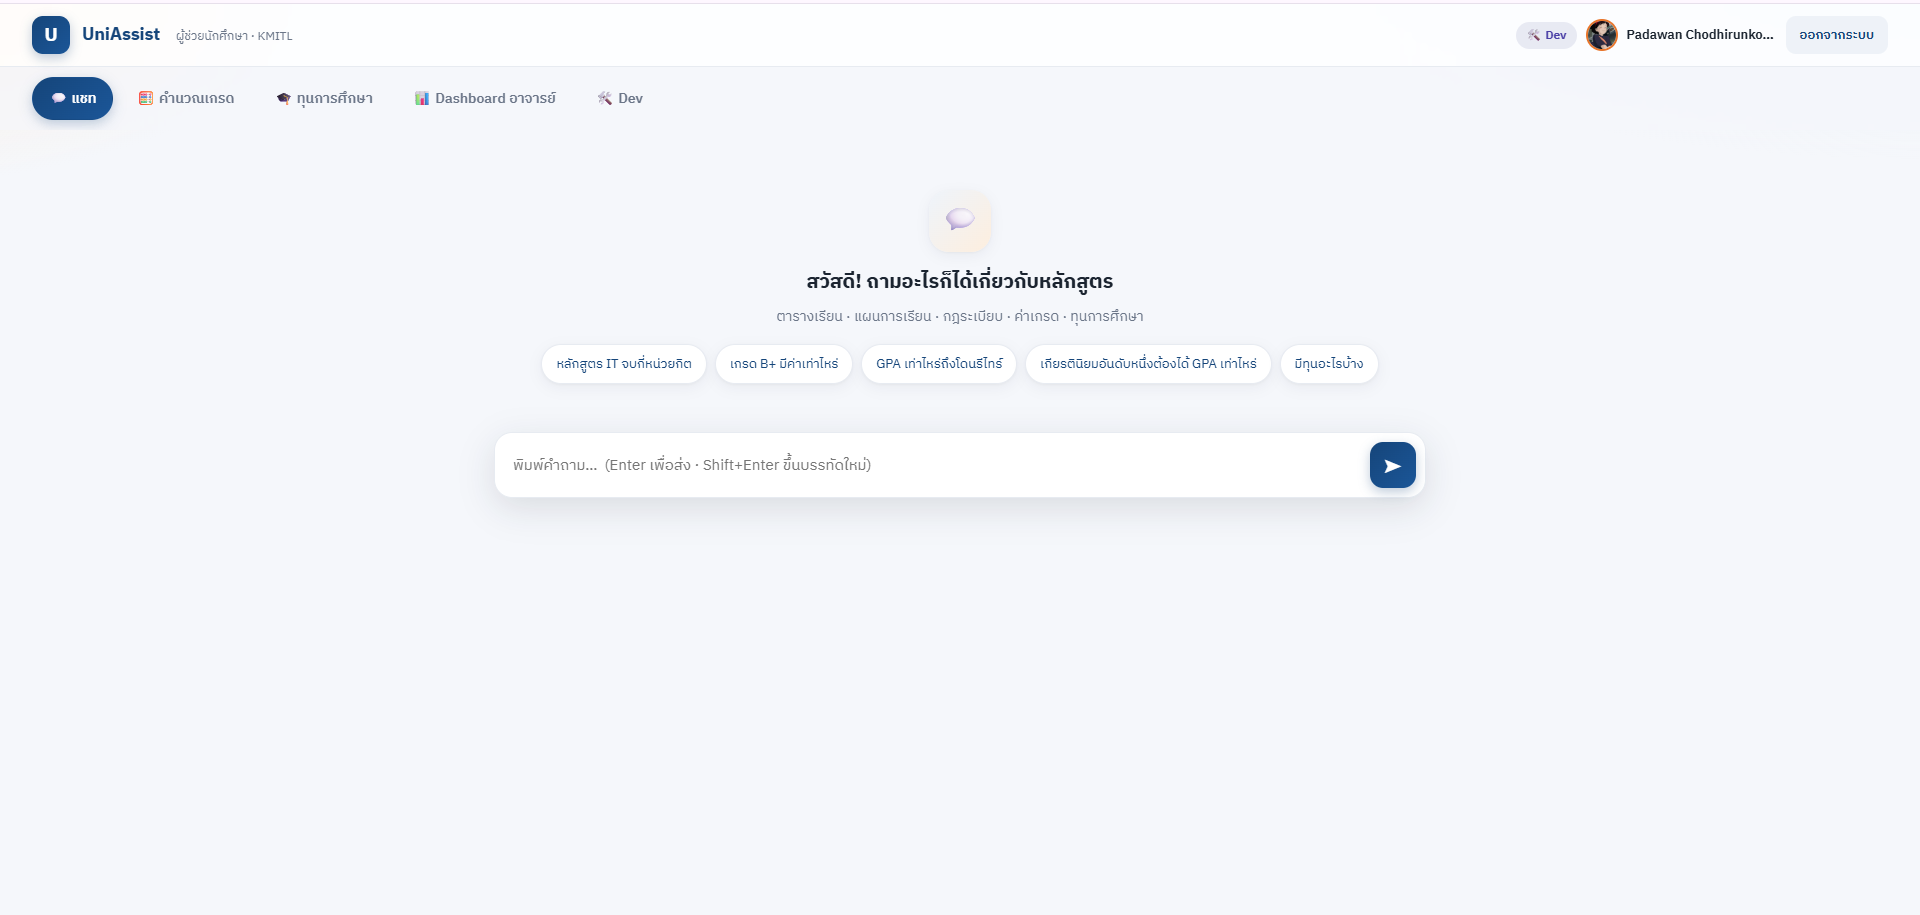
\includegraphics[width=0.95\linewidth]{chat.png}
    \caption{หน้าแชทถาม-ตอบข้อมูลหลักสูตรของระบบ UniAssist AI}
    \label{fig:chat}
\end{figure}

\subsection{หน้าคำนวณเกรดและประเมินความเสี่ยง}

หน้าคำนวณเกรดให้ผู้ใช้วางข้อความผลการเรียนหรือแก้ไขรายวิชาในตาราง ระบบจะคำนวณ GPA รายภาคการศึกษาและสะสม พร้อมจัดสถานะทางการเรียน (เช่น เสี่ยงพ้นสภาพ ภาคทัณฑ์ หรือเข้าเกณฑ์เกียรตินิยม) ดังรูปที่ \ref{fig:gpa}

\begin{figure}[ht]
    \centering
    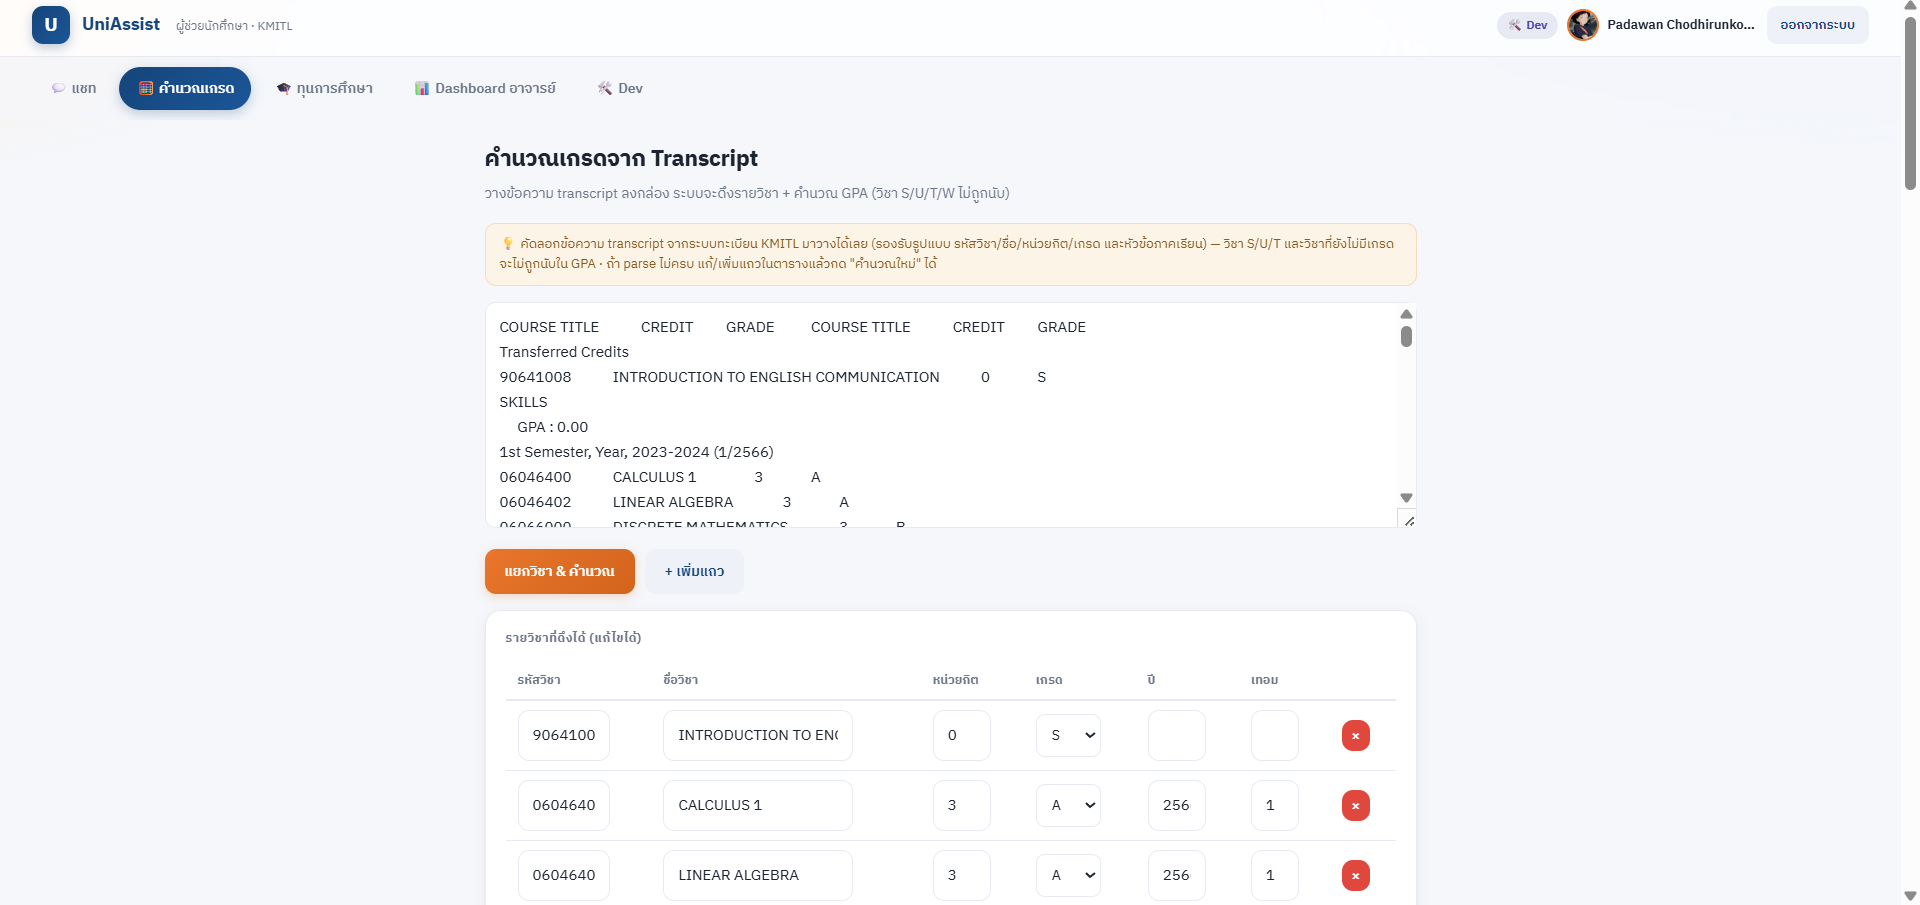
\includegraphics[width=0.95\linewidth]{gpa.png}
    \caption{หน้าคำนวณเกรดและประเมินสถานะทางการเรียน}
    \label{fig:gpa}
\end{figure}

\subsection{หน้าข้อมูลทุนการศึกษา}

หน้าข้อมูลทุนการศึกษาแสดงรายการทุนพร้อมเงื่อนไขและคุณสมบัติ ดังรูปที่ \ref{fig:scholarship}

\begin{figure}[ht]
    \centering
    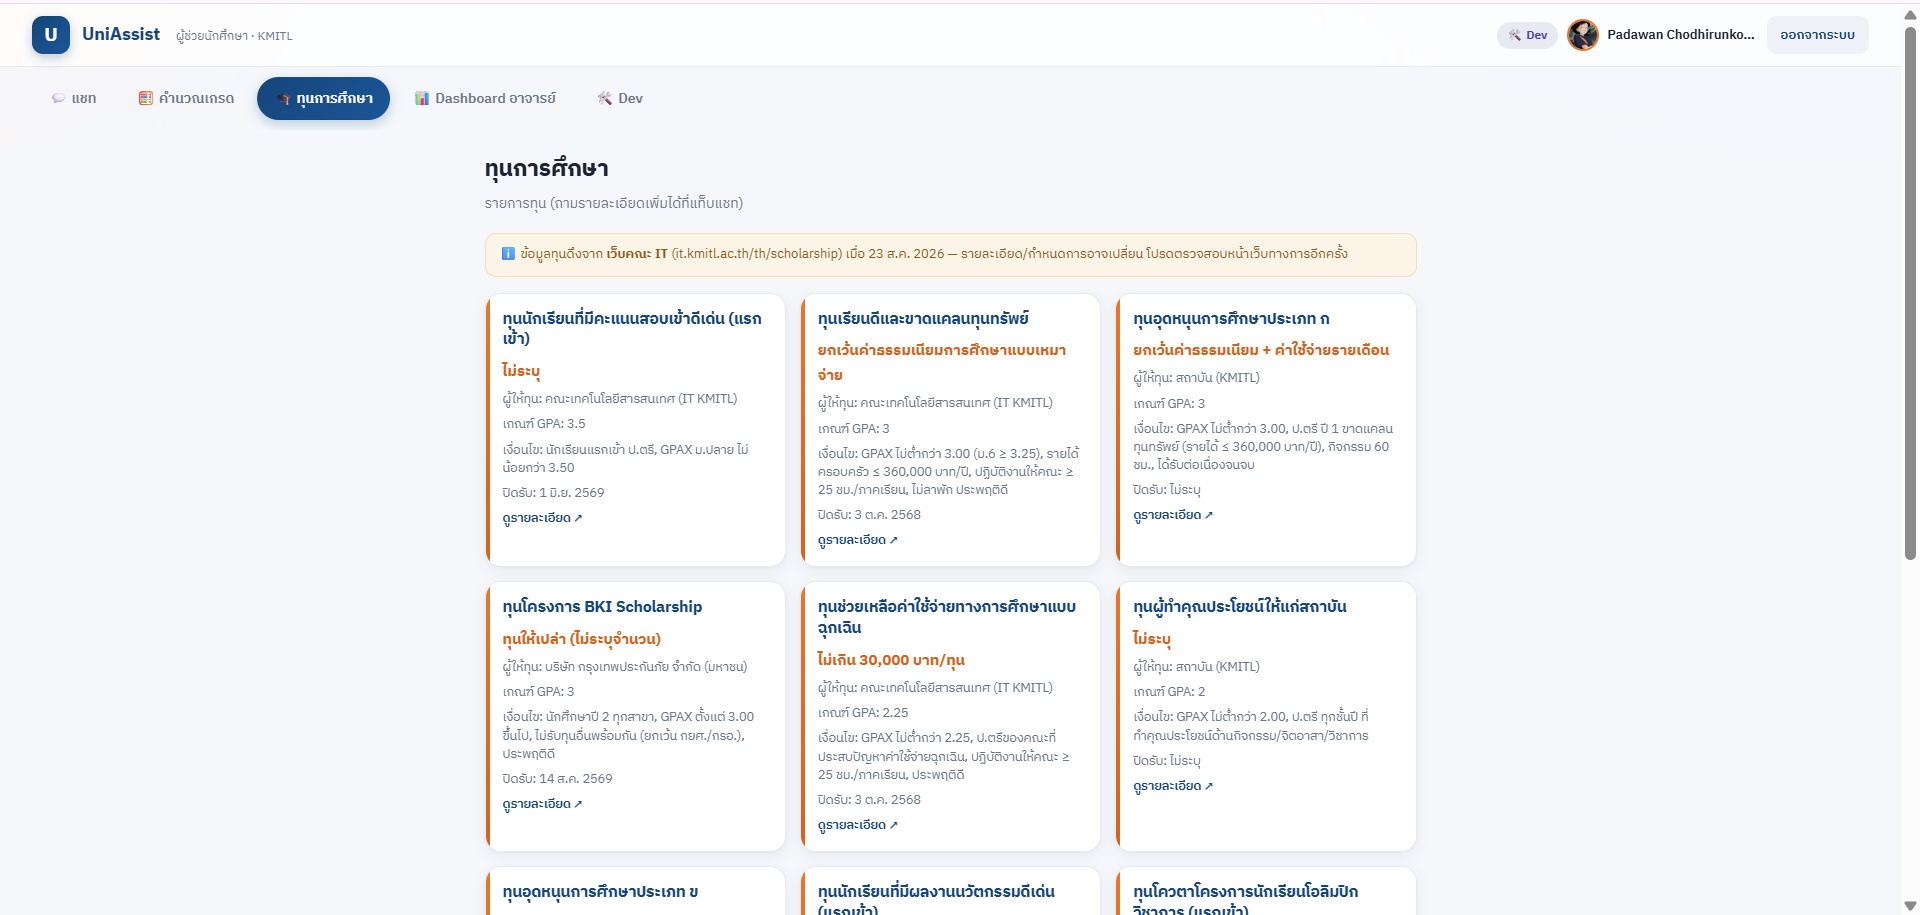
\includegraphics[width=0.95\linewidth]{scholarship.png}
    \caption{หน้าข้อมูลทุนการศึกษา}
    \label{fig:scholarship}
\end{figure}

\section{ผลการสร้างฐานข้อมูล}

จากกระบวนการสกัดและนำเข้าข้อมูล ระบบได้ฐานข้อมูลเชิงสัมพันธ์ที่ครอบคลุมทั้ง 4 หลักสูตรของคณะเทคโนโลยีสารสนเทศ ประกอบด้วยรายวิชา 300 รายวิชา แผนการเรียนรายเทอม 583 รายการ ระเบียบข้อบังคับ 108 รายการ และข้อมูลทุนการศึกษา 11 ทุน ตามที่แสดงในตารางที่ \ref{tab:schema} ของบทที่ \ref{chapter:experiment} ฐานข้อมูลนี้ถูกใช้เป็นแหล่งข้อมูลจริงสำหรับการค้นคืนของแกน Text-to-SQL และการคำนวณต่าง ๆ

\section{ผลการประเมินและคัดเลือกโมเดลภาษาสำหรับการสกัดข้อมูล}

ผลการประเมินคุณภาพการสกัดข้อมูลของโมเดลทั้ง 4 ตัว เทียบกับเอกสาร มคอ.2 ฉบับจริง สรุปได้ดังตารางที่ \ref{tab:model-summary}

\begin{table}[ht]
    \centering
    \caption{สรุปผลการเปรียบเทียบความครบถ้วนและความถูกต้องของการสกัดข้อมูลแต่ละโมเดล}
    \label{tab:model-summary}
    \begin{tabularx}{\linewidth}{l c c c X}
        \toprule
        \textbf{โมเดล} & \textbf{Coverage} & \textbf{Accuracy} & \textbf{แอตทริบิวต์} & \textbf{ข้อสังเกต} \\
        \midrule
        Qwen & 91.7\% & 95.2\% & 7/7 & สมดุลดีที่สุด ครบและแม่น \\
        Gemini & 91.7\% & 89.7\% & 7/7 & ครบดี แต่แม่นรองจาก Qwen \\
        DeepSeek & 93.8\% & 84.9\% & 7/7 & ดึงครบที่สุด แต่แม่นน้อยที่สุด \\
        Typhoon & 55.6\% & 97.3\% & 4/7 & แม่นเมื่อดึงเจอ แต่ดึงพลาดเกือบครึ่ง \\
        \bottomrule
    \end{tabularx}
\end{table}

จากตารางที่ \ref{tab:model-summary} จะเห็นว่าแม้โมเดล Typhoon จะมีความถูกต้อง (Accuracy) สูงที่สุด แต่มีความครบถ้วน (Coverage) เพียง 55.6\% และดึงแอตทริบิวต์ได้เพียง 4 จาก 7 รายการ จึงไม่เหมาะกับการสร้างฐานข้อมูลที่ต้องการความครบถ้วน ส่วนโมเดล DeepSeek แม้ดึงรายวิชาได้ครบที่สุด แต่มีความถูกต้องของค่าต่ำที่สุด ขณะที่โมเดล Qwen ให้ผลที่สมดุลที่สุด คือมีความครบถ้วน 91.7\% ควบคู่กับความถูกต้องสูงถึง 95.2\% และดึงครบทั้ง 7 แอตทริบิวต์ ด้วยเหตุนี้จึงเลือกใช้ \textbf{โมเดล Qwen เป็นโมเดลหลัก} ทั้งในกระบวนการสกัดข้อมูลและการใช้งานจริงในระบบ

ตารางที่ \ref{tab:coverage-curriculum} แสดงความครบถ้วนของการสกัดรายวิชาแยกตามหลักสูตร โดยตัวเลขในวงเล็บคือจำนวนรายวิชาทั้งหมด (Union) ของแต่ละหลักสูตร

\begin{table}[ht]
    \centering
    \caption{ความครบถ้วน (Coverage) ของการสกัดรายวิชาแยกตามหลักสูตร}
    \label{tab:coverage-curriculum}
    \begin{tabularx}{\linewidth}{X c c c c}
        \toprule
        \textbf{หลักสูตร (จำนวนวิชา)} & \textbf{Qwen} & \textbf{Gemini} & \textbf{DeepSeek} & \textbf{Typhoon} \\
        \midrule
        IT (110) & 93.6\% & 90.9\% & 94.5\% & 50.0\% \\
        DSBA (90) & 90.0\% & 91.1\% & 93.3\% & 48.9\% \\
        BIT (69) & 85.5\% & 89.9\% & 89.9\% & 62.3\% \\
        AIT (55) & 98.2\% & 96.4\% & 98.2\% & 69.1\% \\
        \bottomrule
    \end{tabularx}
\end{table}

นอกจากนี้ เมื่อพิจารณาความสอดคล้องของค่าในแต่ละแอตทริบิวต์ (เฉลี่ยรวมทุกหลักสูตร) ดังตารางที่ \ref{tab:attr-agreement} พบว่าแอตทริบิวต์ที่โมเดลสกัดได้แม่นยำที่สุดคือชื่อวิชาภาษาไทย (95.4\%) รองลงมาคือประเภทวิชา (86.3\%) ขณะที่แอตทริบิวต์ที่ท้าทายที่สุดคือปี/ภาคการศึกษา (61.5\%) และหมวดวิชา (63.3\%) เนื่องจากข้อมูลส่วนนี้ในเอกสาร มคอ.2 มักอยู่ในรูปแบบที่ตีความได้หลายแบบ เช่น รายวิชาเลือกที่ลงเรียนได้หลายเทอม

\begin{table}[ht]
    \centering
    \caption{ความสอดคล้องของค่ารายแอตทริบิวต์ (เฉลี่ยรวมทุกหลักสูตร)}
    \label{tab:attr-agreement}
    \begin{tabularx}{\linewidth}{X c}
        \toprule
        \textbf{แอตทริบิวต์} & \textbf{ความสอดคล้องเฉลี่ย} \\
        \midrule
        ชื่อวิชา (ภาษาไทย) & 95.4\% \\
        ประเภทวิชา (บังคับ/เลือก) & 86.3\% \\
        ชื่อวิชา (ภาษาอังกฤษ) & 75.6\% \\
        หน่วยกิต & 74.8\% \\
        หมวดวิชา & 63.3\% \\
        ปี/ภาคการศึกษา & 61.5\% \\
        \bottomrule
    \end{tabularx}
\end{table}

\section{ผลการทดสอบแกน Text-to-SQL}

จากการทดสอบการทำงานของแกน Text-to-SQL พบว่าระบบสามารถแปลงคำถามภาษาไทยเป็นคำสั่ง SQL และตอบคำถามข้อมูลหลักสูตรได้อย่างถูกต้อง เช่น คำถามเกี่ยวกับจำนวนหน่วยกิตที่ต้องเรียนจบของแต่ละหลักสูตร รายวิชาในแผนการเรียนแต่ละเทอม รายวิชาบังคับก่อน และเงื่อนไขระเบียบต่าง ๆ โดยระบบแสดงคำสั่ง SQL ที่ใช้ควบคู่กับคำตอบเสมอ ทำให้สามารถตรวจสอบความถูกต้องได้

กลไกตรวจสอบความปลอดภัยของคำสั่งทำงานได้ตามที่ออกแบบไว้ กล่าวคือ คำสั่งที่ไม่ใช่ \texttt{SELECT}/\texttt{WITH} หรือมีคำสั่งเขียน/แก้ไขข้อมูล จะถูกปฏิเสธก่อนรัน และคำสั่งที่ไม่มี \texttt{LIMIT} จะถูกเติมโดยอัตโนมัติ นอกจากนี้ กลไกสำรอง (Fallback) ช่วยให้ระบบยังตอบผู้ใช้ได้แม้ในกรณีที่ไม่สามารถสร้างคำสั่ง SQL ที่เหมาะสม โดยสลับไปโหมดสนทนาที่ยึดข้อเท็จจริงจากฐานข้อมูล

อย่างไรก็ตาม ในระหว่างการทดสอบพบว่าบริการโมเดลภาษาที่เรียกใช้ผ่านผู้ให้บริการภายนอกมีความไม่คงเส้นคงวา (Nondeterminism) เป็นบางครั้ง กล่าวคือ คำถามเดียวกันอาจได้รับคำตอบ \texttt{NO\_ANSWER} ในบางช่วงเวลาแม้จะเป็นคำถามที่ตอบได้จริง ซึ่งเกิดจากการที่ผู้ให้บริการสลับใช้เซิร์ฟเวอร์ที่มีการบีบอัดโมเดล (Quantization) แตกต่างกัน ปัญหานี้ได้รับการบรรเทาด้วยกลไกการลองสร้างคำสั่งใหม่ (Retry) เมื่อได้ผลลัพธ์ \texttt{NO\_ANSWER} และการเลือกใช้โมเดล Qwen ขนาดใหญ่ที่ให้ผลนิ่งกว่า

\section{ผลการทดสอบระบบคำนวณเกรดและแดชบอร์ด}

ระบบคำนวณเกรดสามารถแยกวิเคราะห์ข้อความผลการเรียนที่มีรูปแบบหลากหลาย คำนวณ GPA รายภาคการศึกษาและสะสมได้ถูกต้อง โดยตัดรายวิชาที่ไม่นับหน่วยกิต GPA ออกอย่างเหมาะสม และจัดสถานะทางการเรียนตามเกณฑ์ที่อ้างอิงจากฐานข้อมูลจริง ส่วนแดชบอร์ดสำหรับอาจารย์ที่ปรึกษาสามารถแสดงภาพรวมผลการเรียนเฉลี่ยรายภาคของนักศึกษาในความดูแล และจำแนกกลุ่มความเสี่ยงได้ตามที่ออกแบบไว้ ช่วยให้อาจารย์สามารถระบุนักศึกษาที่ควรได้รับการดูแลเป็นพิเศษได้อย่างรวดเร็ว

    \chapter{บทสรุป}
\label{chapter:conclusion}

\section{สรุปผลการดำเนินงาน}

โครงงานนี้ได้พัฒนา UniAssist AI ซึ่งเป็นเว็บแอปพลิเคชันผู้ช่วยด้านวิชาการสำหรับนักศึกษาและอาจารย์ที่ปรึกษา คณะเทคโนโลยีสารสนเทศ สถาบันเทคโนโลยีพระจอมเกล้าเจ้าคุณทหารลาดกระบัง โดยมีเป้าหมายเพื่อรวบรวมข้อมูลทางการศึกษาที่กระจัดกระจายให้อยู่ในศูนย์กลางเดียว และให้บริการตอบคำถามด้านวิชาการได้อย่างถูกต้องและรวดเร็ว

ผลการดำเนินงานสามารถสรุปตามวัตถุประสงค์ได้ดังนี้

\begin{enumerate}
    \item \textbf{การรวบรวมและสร้างฐานข้อมูล} ระบบสามารถสกัดข้อมูลหลักสูตรจากเอกสาร มคอ.2 ด้วยโมเดลภาษาขนาดใหญ่ และจัดเก็บลงในฐานข้อมูลเชิงสัมพันธ์ที่ครอบคลุมทั้ง 4 หลักสูตร โดยมีการประเมินคุณภาพการสกัดเทียบกับเอกสารจริง และเลือกใช้โมเดล Qwen ที่ให้ผลสมดุลที่สุด (Coverage 91.7\%, Accuracy 95.2\%)
    \item \textbf{การพัฒนา AI Chatbot} ระบบใช้เทคนิค Text-to-SQL ในการแปลงคำถามภาษาไทยเป็นคำสั่ง SQL และตอบคำถามโดยอ้างอิงจากข้อมูลจริงในฐานข้อมูล พร้อมกลไกตรวจสอบความปลอดภัยของคำสั่งและกลไกสำรอง ทำให้คำตอบสามารถตรวจสอบย้อนกลับได้และลดปัญหาการสร้างข้อมูลเท็จ
    \item \textbf{การคำนวณเกรดและประเมินความเสี่ยง} ระบบสามารถคำนวณ GPA และประเมินสถานะทางการเรียนโดยอัตโนมัติ โดยอ้างอิงค่าเกรดและเกณฑ์จากฐานข้อมูล ไม่ใช้ค่าคงที่
    \item \textbf{ระบบทุนการศึกษาและแดชบอร์ดอาจารย์} ระบบให้ข้อมูลทุนการศึกษาและช่วยวิเคราะห์คุณสมบัติเบื้องต้น พร้อมแดชบอร์ดที่ช่วยให้อาจารย์ที่ปรึกษาติดตามภาพรวมและความเสี่ยงของนักศึกษาในความดูแลได้
    \item \textbf{การยืนยันตัวตนและความปลอดภัย} ระบบมีการยืนยันตัวตนผ่าน Google OAuth และแบ่งสิทธิ์ตามบทบาท ควบคู่กับการจำกัดการเข้าถึงฐานข้อมูลแบบอ่านอย่างเดียว
\end{enumerate}

\section{อภิปรายผล}

ผลการดำเนินงานแสดงให้เห็นว่าการเลือกวิธีการค้นคืนข้อมูลควรพิจารณาจากลักษณะของข้อมูลเป็นสำคัญ เนื่องจากข้อมูลหลักสูตรมีโครงสร้างที่ชัดเจน การใช้เทคนิค Text-to-SQL บนฐานข้อมูลเชิงสัมพันธ์จึงให้คำตอบที่แม่นยำ ตรวจสอบย้อนกลับได้ และลดปัญหาการสร้างข้อมูลเท็จได้ดีกว่าการให้โมเดลภาษาตอบจากความจำโดยตรง อีกทั้งการออกแบบให้โมเดลภาษาเป็นเพียงผู้สร้างคำสั่งค้นข้อมูล ไม่ใช่ผู้เก็บข้อเท็จจริง ทำให้ระบบมีความน่าเชื่อถือมากขึ้น

นอกจากนี้ ผลการประเมินการสกัดข้อมูลยังชี้ให้เห็นว่าไม่มีโมเดลใดที่ดีที่สุดในทุกมิติ การพิจารณาทั้งความครบถ้วนและความถูกต้องควบคู่กันจึงมีความสำคัญในการเลือกโมเดลให้เหมาะกับงาน

\section{ข้อจำกัดของระบบ}

\begin{enumerate}
    \item \textbf{ความไม่คงเส้นคงวาของบริการโมเดลภาษา} การเรียกใช้โมเดลผ่านผู้ให้บริการภายนอกอาจให้ผลลัพธ์ที่ไม่นิ่งเป็นบางครั้ง (เช่น ตอบ \texttt{NO\_ANSWER} แม้ตอบได้จริง) ซึ่งบรรเทาได้ด้วยกลไกลองใหม่และการเลือกโมเดลที่นิ่งกว่า แต่ยังไม่สามารถขจัดได้ทั้งหมด
    \item \textbf{ความครบถ้วนของการสกัดข้อมูล} รายวิชาบางประเภท เช่น วิชาเลือกเสรีหรือวิชาที่ใช้รหัส placeholder ในเอกสาร มคอ.2 ยังถูกสกัดได้ไม่ครบถ้วนสมบูรณ์
    \item \textbf{ขอบเขตของข้อมูล} ระบบครอบคลุมเฉพาะข้อมูลหลักสูตรของคณะเทคโนโลยีสารสนเทศ และข้อมูลนักศึกษาตัวอย่างที่ใช้ทดสอบยังมีจำนวนจำกัด
    \item \textbf{การค้นคืนข้อมูลเชิงบรรยาย} ระเบียบหรือประกาศที่อยู่ในรูปแบบข้อความยาวและไม่มีโครงสร้างชัดเจน ยังไม่ได้รับการค้นคืนด้วยเทคนิคเชิงความหมาย (Semantic Search) อย่างเต็มรูปแบบ
\end{enumerate}

\section{ข้อเสนอแนะและแนวทางการพัฒนาต่อ}

\begin{enumerate}
    \item เพิ่มการค้นคืนข้อมูลแบบ Retrieval-Augmented Generation ด้วยฐานข้อมูลเชิงเวกเตอร์ สำหรับข้อมูลเชิงบรรยายที่ไม่มีโครงสร้างชัดเจน เพื่อเสริมการทำงานของแกน Text-to-SQL ที่เหมาะกับข้อมูลเชิงโครงสร้าง
    \item เชื่อมต่อกับระบบทะเบียนของสถาบันโดยตรง เพื่อให้ข้อมูลผลการเรียนและตารางเรียนของนักศึกษาเป็นปัจจุบันแบบอัตโนมัติ
    \item ขยายฟังก์ชันการแนะนำรายวิชาและการตรวจสอบตารางเรียน (Schedule Conflict) ให้สมบูรณ์ยิ่งขึ้น
    \item ขยายชุดข้อมูลนักศึกษาและจัดทำการประเมินประสิทธิภาพการตอบคำถามของระบบกับผู้ใช้จริงในวงกว้าง
    \item พิจารณาปรับจูนโมเดลภาษา (Fine-tuning) ด้วยชุดคำถาม-คำสั่ง SQL เฉพาะโดเมนของสถาบัน เพื่อเพิ่มความแม่นยำและลดการพึ่งพาบริการภายนอก
\end{enumerate}

\section{สรุป}

โดยรวม UniAssist AI สามารถบรรลุวัตถุประสงค์ที่ตั้งไว้ในการเป็นเครื่องมือช่วยให้นักศึกษาเข้าถึงข้อมูลและวางแผนการเรียนได้อย่างมีประสิทธิภาพ ลดความเสี่ยงในการพ้นสภาพนักศึกษา และช่วยให้อาจารย์ที่ปรึกษาติดตามดูแลนักศึกษาได้อย่างทั่วถึง ซึ่งสอดคล้องกับเป้าหมายการพัฒนาที่ยั่งยืน SDG 4 ในการส่งเสริมโอกาสการเรียนรู้และคุณภาพการศึกษาอย่างเท่าเทียม


    \clearpage

    \def\inbib{1}
    \addcontentsline{toc}{chapter}{\bibname}
    \bibliographystyle{IEEEtran-kmitl}
    \makeatletter
    \EveryShipout{
        \ifdim\pagetotal>\pagegoal
            \if\inbib1
                \aftergroup\@cont@heading
            \else
            \fi
        \fi
    }
    \makeatother

    \bibliography{reference}
    \def\inbib{0}

    \startappendix
    \chapter{ตัวอย่างการทำงานของระบบ Text-to-SQL}

ภาคผนวกนี้แสดงตัวอย่างคำถามภาษาไทยของผู้ใช้ คู่กับคำสั่ง SQL ที่โมเดลภาษาสร้างขึ้นและนำไปประมวลผลบนฐานข้อมูล เพื่อให้เห็นภาพการทำงานจริงของแกน Text-to-SQL

\vskip0.5cm
\noindent\textbf{ตัวอย่างที่ 1} คำถาม: ``หลักสูตร IT ต้องเรียนกี่หน่วยกิตถึงจะจบ''

\begin{verbatim}
SELECT program_code, total_credits
FROM programs
WHERE program_code = 'IT';
\end{verbatim}

\noindent\textbf{ตัวอย่างที่ 2} คำถาม: ``วิชาบังคับก่อนของวิชารหัส 06016418 มีอะไรบ้าง''

\begin{verbatim}
SELECT cp.prerequisite_code
FROM course_prerequisites cp
JOIN courses c ON c.course_id = cp.course_id
WHERE c.code = '06016418';
\end{verbatim}

\noindent\textbf{ตัวอย่างที่ 3} คำถาม: ``แผนการเรียนปกติของ IT ปี 1 เทอม 1 มีวิชาอะไรบ้าง''

\begin{verbatim}
SELECT apc.code, apc.name_th, apc.credits_total
FROM academic_plan_courses apc
JOIN programs p ON p.program_id = apc.program_id
WHERE p.program_code = 'IT'
  AND apc.plan_type = 'no_coop'
  AND apc.year = 1
  AND apc.semester = 1;
\end{verbatim}

\noindent\textbf{ตัวอย่างที่ 4} คำถาม: ``เกณฑ์การพ้นสภาพ (รีไทร์) เป็นอย่างไร''

\begin{verbatim}
SELECT category, text
FROM rules
WHERE category = 'dismissal_criteria'
  AND text LIKE '%เฉลี่ยสะสม%';
\end{verbatim}


    \makeauthorbio

\end{document}
